%%%%%%%%%%%%%%%%%%%%%%%%%%%%%%%%%%%%%%%%%%%%%%%%%
%    			Imperial College			    %
%			Department of Materials			    %
% Materials Characterisation Report Template    %
%%%%%%%%%%%%%%%%%%%%%%%%%%%%%%%%%%%%%%%%%%%%%%%%%
% CHANGES                                       %
%   -Updated to use Helvetica font              %
%%%%%%%%%%%%%%%%%%%%%%%%%%%%%%%%%%%%%%%%%%%%%%%%%



\documentclass[twoside,10pt,a4paper]{article}
%describes the document we are making

%%%%%%%%%%%%%%%%%%%%%%%%%%%%%%%%%%%%%%%% 
%Document preamble, adds useful packages and sets up the document. 


%FONT AND TYPESETTING
\usepackage[french]{babel}							%makes latex aware of your language, so better hyphenating etc
\usepackage[T1]{fontenc} 							%use the T1 for proper searching and use of ligatures etc
\usepackage[utf8]{inputenc}							%use UTF8 encoding for reading source code
\usepackage{helvet}								%use the helvetica font. This is very similar to the Arial font used in the Office templates.
\renewcommand{\familydefault}{\sfdefault}
\usepackage{microtype}								%enables microtypesetting
\usepackage{blindtext}
\usepackage{csquotes}

%PAGE LAYOUT
\usepackage[onehalfspacing]{setspace}				%adjusts linespacing
\usepackage{geometry}				                %adjusts page layout including margins
\geometry{left=2cm,right=2cm,top=3cm,bottom=3cm}	%the page geometry as defined, A4=210x297mm
\pagestyle{plain}						            %includes page number in centred in footer


%MATHS
\usepackage{mathtools} 								%for the rendering of maths
\numberwithin{equation}{section}					%reset numbering within a structural object
\numberwithin{figure}{section}						%reset numbering within a structural object
\usepackage{amsmath}

%SCIENCE
\usepackage[version=4]{mhchem}						%typesetting of chemical formulae
\usepackage{siunitx}								%typesetting of units and quantities with uncertainties etc
\sisetup{detect-all, detect-weight=true, detect-family=true}  %  if the rest of the text is bold the units will be as well
\sisetup{range-units=single}  						% don't include units in both parts of an \SIrange 
\sisetup{multi-part-units=single}					% don't repeat units for multi-part numbers such as numbers with uncertainties
\sisetup{separate-uncertainty}						%list values with uncertanties as X\pm Y rather than X(Y).

%FIGURES AND TABLES
\usepackage{caption}
\usepackage{graphicx}								%for the rendering of floating graphics
\usepackage{float}
\usepackage[section]{placeins}						%defines float barriers at the end of sections. Set option [section] for this.
\usepackage{array} 								%for creating tables
\usepackage{booktabs}								%professional looking tables, provides /toprule etc



%BIBLIOGRAPHY
\usepackage[backend=biber,citestyle=numeric-comp,bibstyle=numeric,sorting=none,url=false,eprint=false,isbn=true,doi=true]{biblatex}
\addbibresource{./example.bib}	%the absolute or relative path of your bibliography file.
\usepackage{hyperref, bookmark}						%turns the references and citations into hyperlinks. This needs to be last on the preamble.
\hypersetup{colorlinks=true,linkcolor=black,citecolor=blue,urlcolor=blue}

%%%%%%%%%%%%%%%%%%%%%%%%%%%%%%%%%%%%%%%%%%%%%%%%%%%%%%%%


\begin{document}
%	Put the document stuff in here!
\fontfamily{phv}\selectfont
\begin{titlepage}			%makes a title page. Remember to change the author, CID, username and group number to what is appropriate for you!
	\centering
	{\scshape\LARGE Univeristé de Lille\par}
	{\scshape \LARGE M1 Informatique - Machine Learning\par}
	\vspace{1cm}
	{\huge\bfseries Rendu Atelier \#2 \par}
	{\huge\bfseries Descente de gradient \par}
	{\huge\bfseries (quasi-)Newton methode (Ordre 1 + Ordre 2) \par}
	\vspace{5cm}
	{\Large\itshape Selim Lakhdar \hfill Phillipe Lesueur \par}		%remember to change these!
	\vspace{5cm}
	%		{\large Group \@group\unskip\strut\par}
	%       \vspace{5cm}
	{\large \today\par}
\end{titlepage}

% LES FONCTIONS
\section{Les fonctions}\label{sec:section1}
Les fonctions étudiées sont toutes proportionelle au paramètre $\alpha$ et elles s'annulent toutes au point 0. 
\subsection{Fonction 1}\label{sec:subsection1}
\begin{equation}
    f_1^{\alpha}(x) = \alpha\sum_{i=1}^{n} x_i^2
    \label{eq:simple}		%these can be labelled too
\end{equation}
\begin{figure}[H]
    \centering
    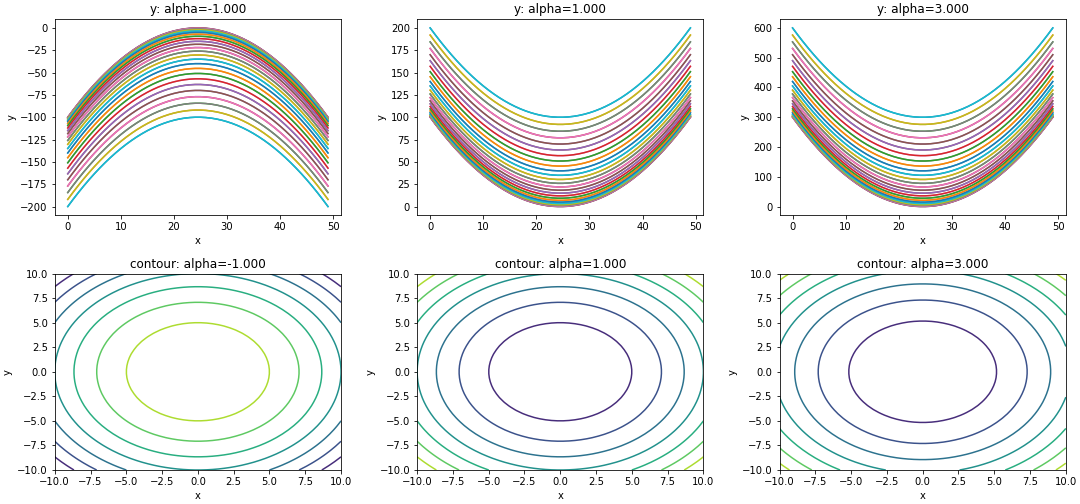
\includegraphics[width=\textwidth]{imgs/contours/f_1_texpres}
    \caption{$f_1^{\alpha}(x)$ y }
    \label{fig:mesh1}
\end{figure}
\subsection{Fonction 2}\label{sec:subsection1}
\begin{equation}
    f_2(x) = \frac{1}{2} \sum_{i=1}^{n} 10^{\alpha \frac {i-1} {n-1}}.x_i^2
    \label{eq:simple}		%these can be labelled too
\end{equation}
\begin{figure}[H]
    \centering
    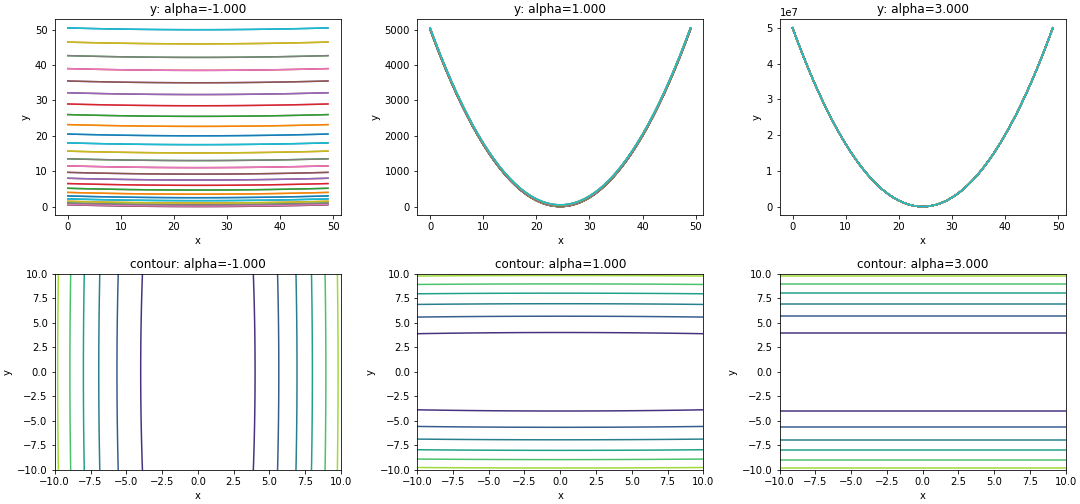
\includegraphics[width=\textwidth]{imgs/contours/f_2_texpres}
    \caption{$f_1^{\alpha}(x)$ y }
    \label{fig:mesh1}
\end{figure}
\subsection{Fonction 3}\label{sec:subsection1}
\begin{equation}
f_3(x) = 10.n + \sum_{i=1}^{n} (10^{\alpha \frac {i-1} {n-1}}.(x_i - 1)^2 - 10.\cos(2\pi(x_i - 1)))
\label{eq:simple}		%these can be labelled too
\end{equation}
\begin{figure}[H]
    \centering
    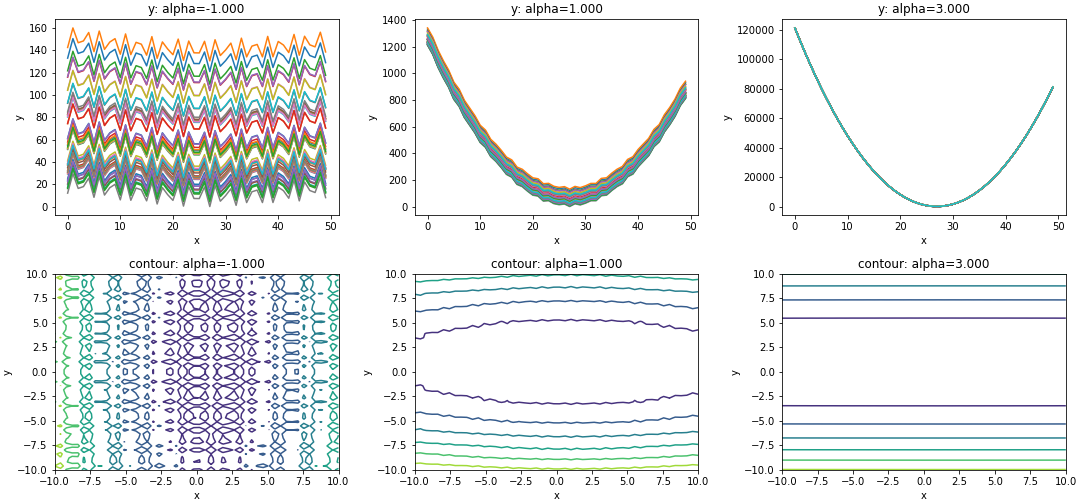
\includegraphics[width=\textwidth]{imgs/contours/f_3_texpres}
    \caption{$f_1^{\alpha}(x)$ y }
    \label{fig:mesh1}
\end{figure}
\subsection{Fonction 4}\label{sec:subsection1}
\begin{equation}
f_4(x) = \sum_{i=1}^{n} (10^{\alpha}.((x_i - 1)^2 - (x_{i+1} - 1))^2 + (x_i - 2)^2)
\label{eq:simple}		%these can be labelled too
\end{equation}
\begin{figure}[H]
    \centering
    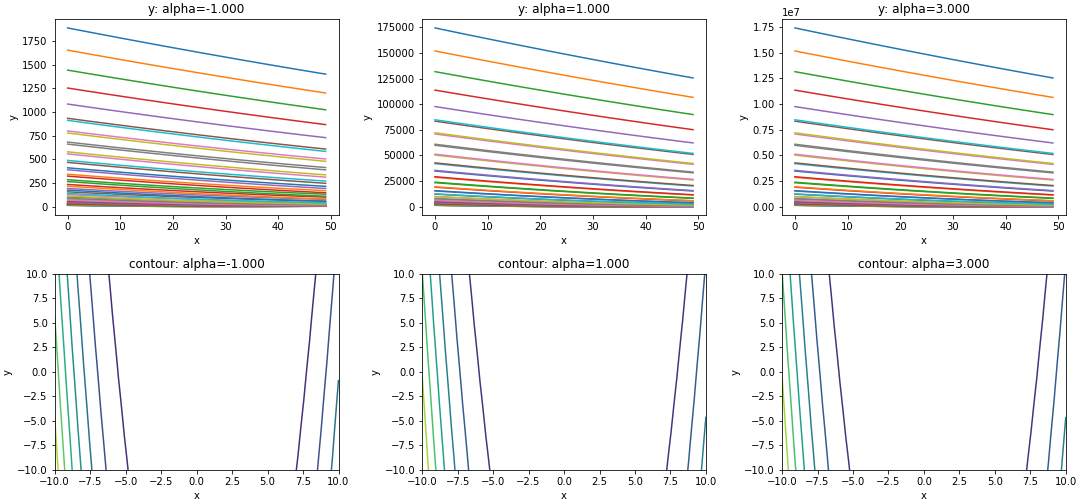
\includegraphics[width=\textwidth]{imgs/contours/f_4_texpres}
    \caption{$f_1^{\alpha}(x)$ y }
    \label{fig:mesh1}
\end{figure}
% GD: FIXED SZ
\section{Gradient Descent: Fixed Step Size}\label{sec:section2}
Dans cette partie nous allons observer une descente de gradient avec un step size fixé. Pour cela nous devons calcluer les dérivées de chaque fonctions: 
\begin{equation}
    f_1'^{\alpha}(x) = \alpha\sum_{i=1}^{n} 2x_i
    \label{eq:simple}		%these can be labelled too
\end{equation}
\begin{equation}
    f_2'(x) = \sum_{i=1}^{n} 10^{\alpha \frac {i-1} {n-1}}.x_i
    \label{eq:simple}		%these can be labelled too
\end{equation}
\begin{equation}
    f_3'(x) = \sum_{i=1}^{n} (10^{\alpha \frac {i-1} {n-1}}2.(x_i - 1) + 10.2\pi\sin(2\pi(x_i - 1)))
    \label{eq:simple}		%these can be labelled too
\end{equation}
\begin{sloppypar}
\begin{equation}
    f_4'(x) =
    \begin{cases} 
    \sum_{i=1}^{n} 4.10^{\alpha}.(xi - 1)((x_i-1)^2 - (x_{i+1} - 1)) + 2(x_i - 2) & x = 0 \\
    \sum_{i=1}^{n} 4.10^{\alpha}.(xi-1)((x_i-1)^2-(x_{i+1}-1))+2(x_i-2)+\sum_{i=1}^{n} -2.10^{\alpha}((x_i-1)^2 - (x_{i+1} - 1)) & 0 < x < n \\
    \sum_{i=1}^{n} -2.10^{\alpha}((x_i-1)^2 - (x_{i+1} - 1)) & x = n 
    \end{cases}
    \label{eq:simple}		%these can be labelled too
\end{equation}
\end{sloppypar}

Par la suite nous allons observer l'évolution des X pendant la déscente du gradiant. Ainsi que les différentes valeurs de Y.
Nous avons choisit d'exposer ici les variantes avec les valeurs min et max de alpha $0.005$ et $3$, vous retrouverez dans le notebook l'intégralité des observations.

\subsection{Fonction 1 }\label{sec:subsection2}
\begin{figure}[H]
    \centering
    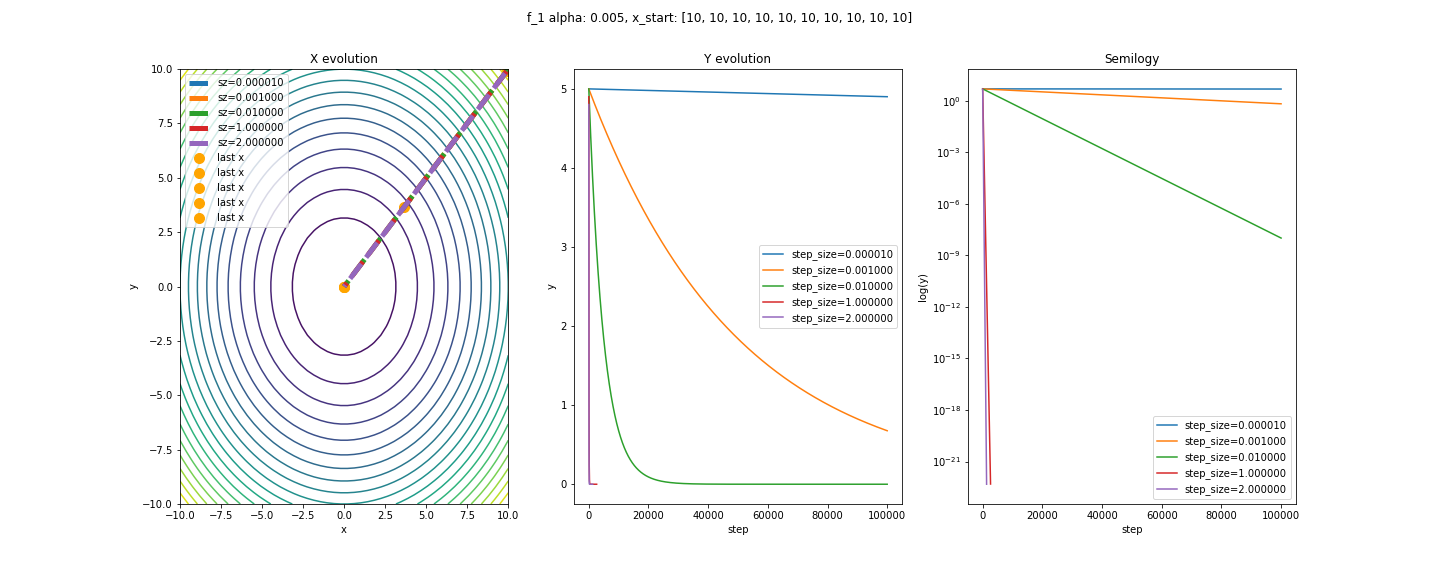
\includegraphics[width=\textwidth]{imgs/fixed_sz/f_1_a-0.005_fixed_sz.png}
    \caption{}
\end{figure}
\begin{figure}[H]
    \centering
    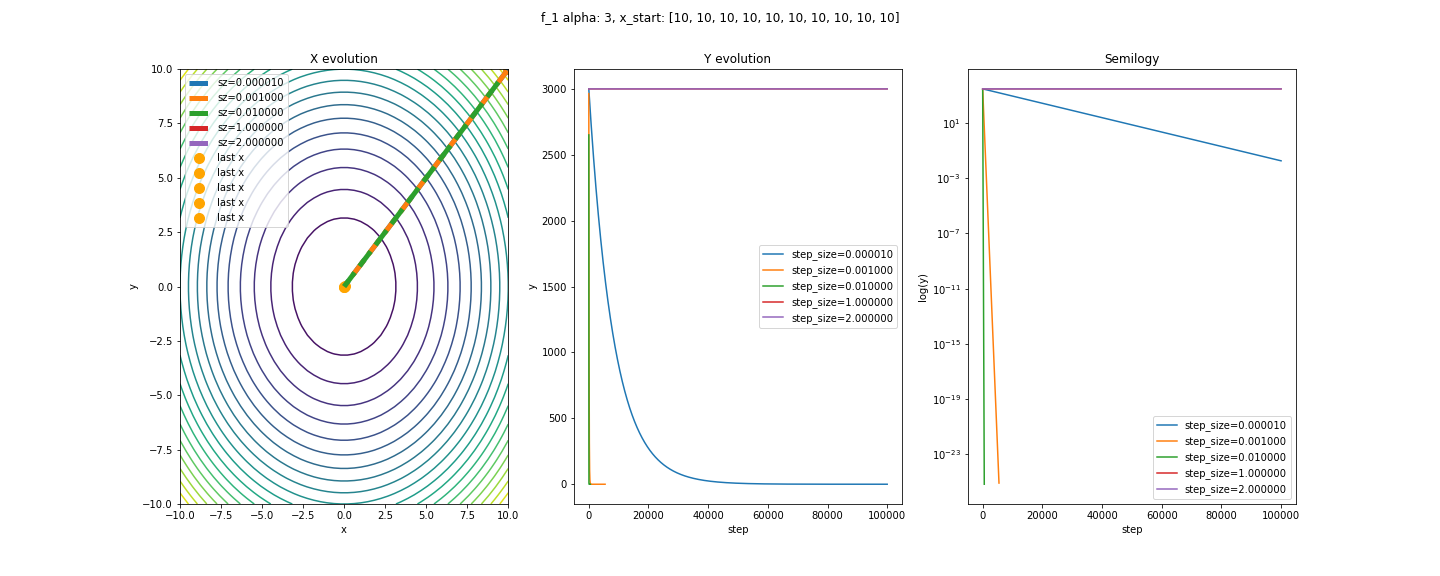
\includegraphics[width=\textwidth]{imgs/fixed_sz/f_1_a-3_fixed_sz.png}
    \caption{}
\end{figure}
\begin{itemize}
	\item La fonction $f_1^{\alpha}(x)$ reste assez simple (fonction convexe) ce qui permet de converger assez simplement.
	\begin{itemize}
    	\item Même en complexifiant la fonction (ie: en prenant une grande valeur de $\alpha$) on arrive à converger.
	\end{itemize}
	\item Cependant on remarque que dans certains cas il nous faut plusieurs itérations.
	\begin{itemize}
    	\item Cela peut être expliqué par des sauts trop grand ou trop petit à cause du $step\_size$
	\end{itemize}
\end{itemize}
\subsection{Fonction 2 }\label{sec:subsection2}
\begin{figure}[H]
    \centering
    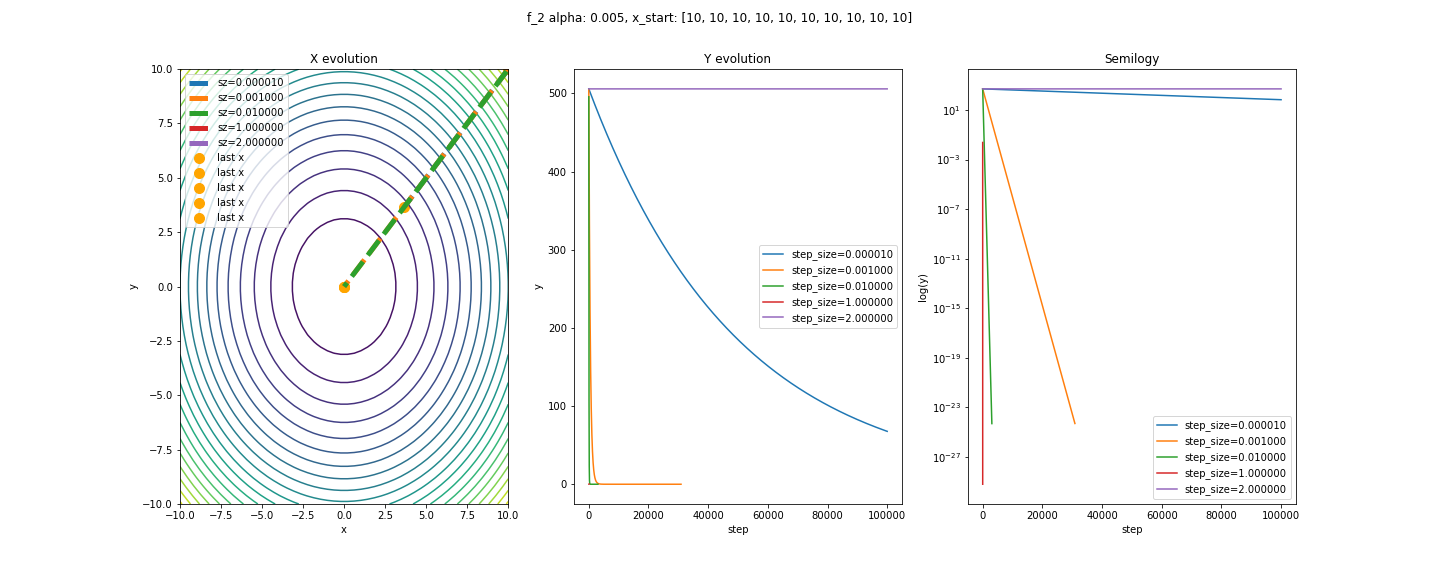
\includegraphics[width=\textwidth]{imgs/fixed_sz/f_2_a-0.005_fixed_sz.png}
    \caption{}
\end{figure}
\begin{figure}[H]
    \centering
    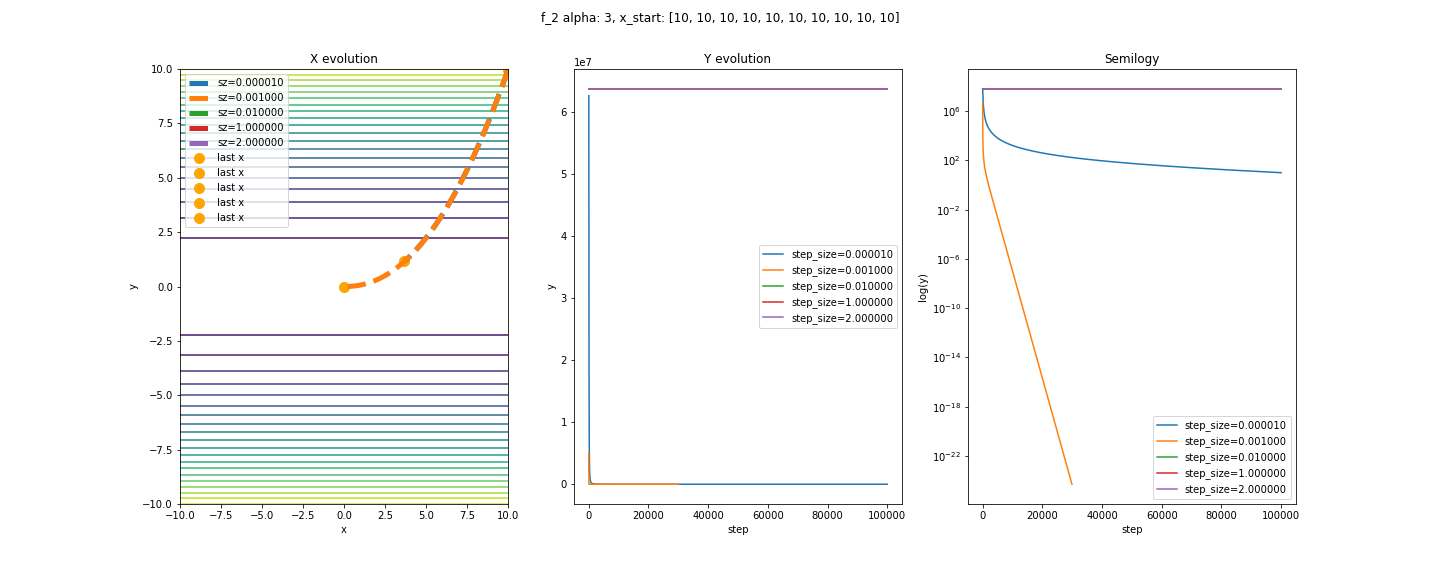
\includegraphics[width=\textwidth]{imgs/fixed_sz/f_2_a-3_fixed_sz.png}
    \caption{}
\end{figure}
\begin{itemize}
	\item La fonction $f_2^{\alpha}(x)$ reste assez simple (fonction convexe) ce qui permet de converger assez simplement.
	\begin{itemize}
    	\item Même en complexifiant la fonction (ie: en prenant une grande valeur de $\alpha$) on arrive à converger.
	\end{itemize}
	\item Cependant on remarque que dans certains cas il nous faut plusieurs itérations.
	\begin{itemize}
    	\item Cela peut être expliqué par des sauts trop grand ou trop petit à cause du $step\_size$
	\end{itemize}
\end{itemize}
\subsection{Fonction 3 }\label{sec:subsection2}
\begin{figure}[H]
    \centering
    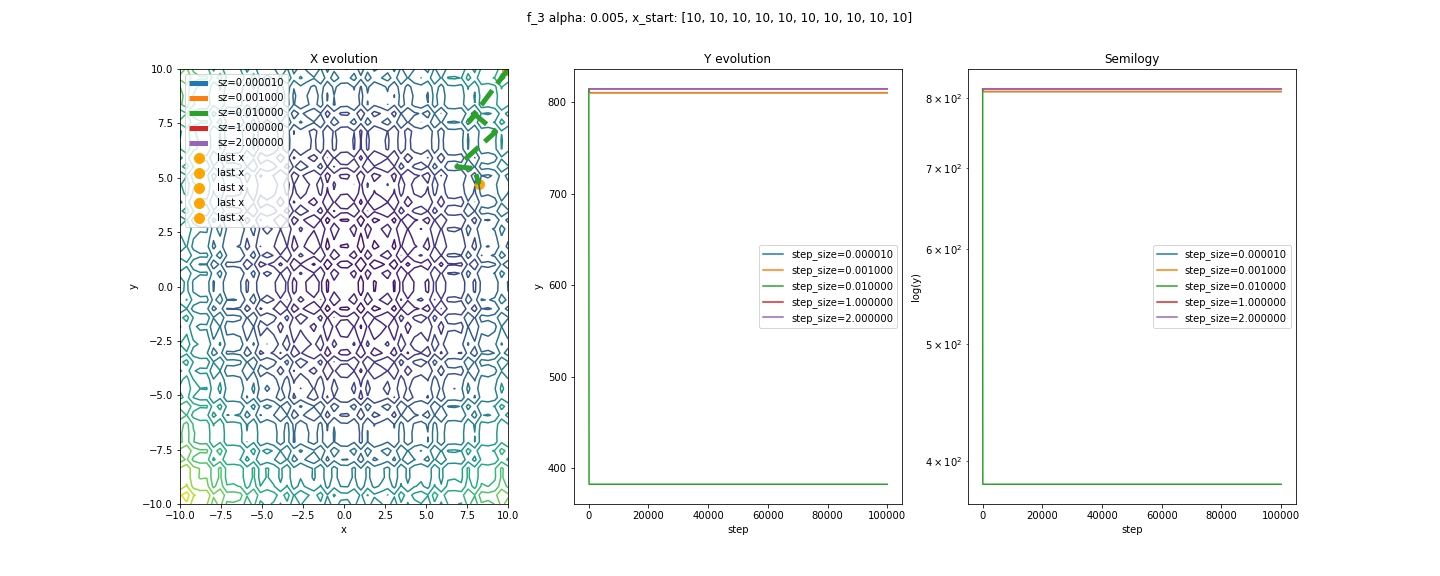
\includegraphics[width=\textwidth]{imgs/fixed_sz/f_3_a-0.005_fixed_sz.png}
    \caption{}
\end{figure}
\begin{figure}[H]
    \centering
    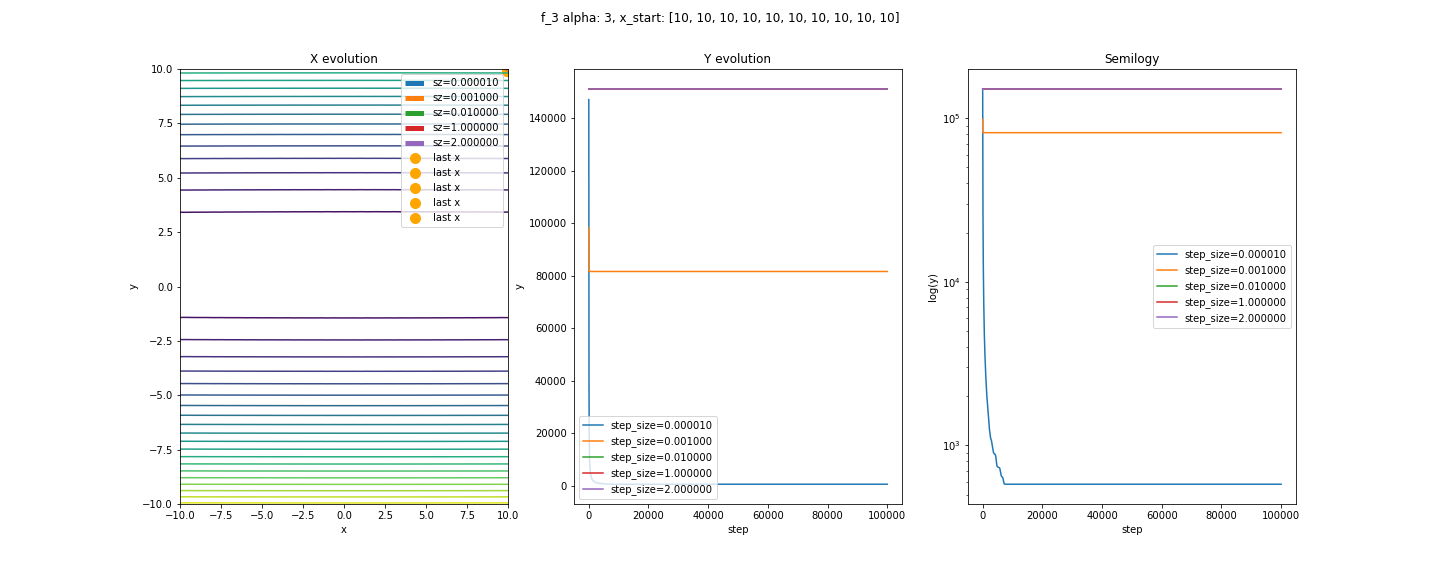
\includegraphics[width=\textwidth]{imgs/fixed_sz/f_3_a-3_fixed_sz.png}
    \caption{}
\end{figure}
\begin{itemize}
	\item La fonction $f_3^{\alpha}(x)$ est plus complexe que les deux dernières (admet plusieurs minimums locaux).
	\begin{itemize}
    	\item En complexifiant la fonction (ie: en prenant une grande valeur de $\alpha$) on ne converge pas.
	\end{itemize}
	\item On remarque que l'agorithme peine à converger, on reste encore loin du minimum (0).
	\begin{itemize}
    	\item On pourrait augmenter le nombre d'itération, mais çela va prendre beaucoup plus de temps.
	\end{itemize}
\end{itemize}
\subsection{Fonction 4 }\label{sec:subsection2}
\begin{figure}[H]
    \centering
    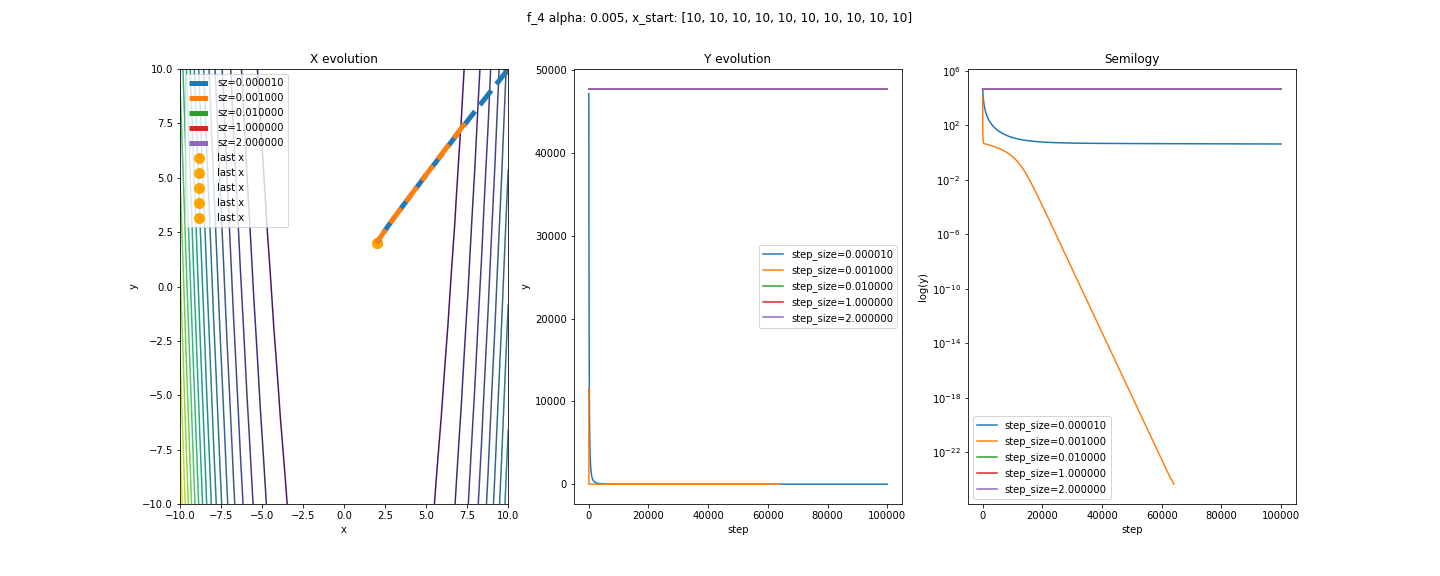
\includegraphics[width=\textwidth]{imgs/fixed_sz/f_4_a-0.005_fixed_sz.png}
    \caption{}
\end{figure}
\begin{figure}[H]
    \centering
    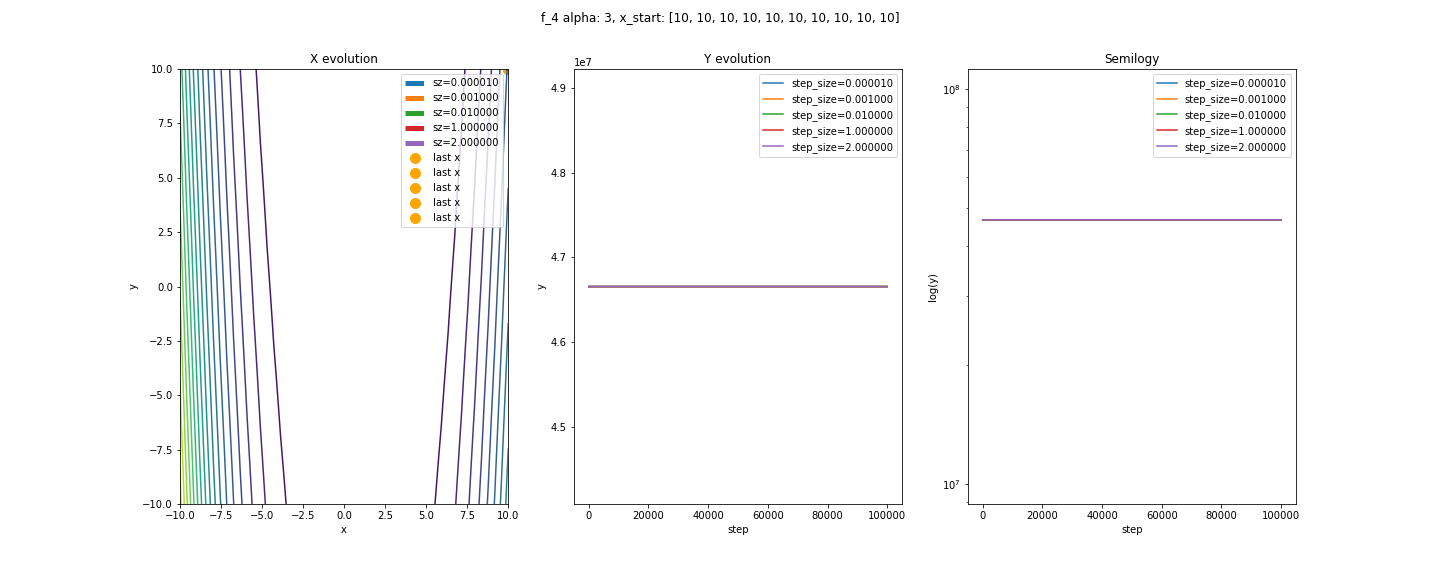
\includegraphics[width=\textwidth]{imgs/fixed_sz/f_4_a-3_fixed_sz.png}
    \caption{}
\end{figure}
\begin{itemize}
	\item La fonction $f_4^{\alpha}(x)$ est la plus complexe (admet plusieurs minimums locaux).
	\begin{itemize}
    	\item En complexifiant la fonction (ie: en prenant une grande valeur de $\alpha$) on ne converge pas.
	\end{itemize}
	\item On remarque que l'agorithme peine à converger, on reste encore loin du minimum (0).
	\begin{itemize}
    	\item On pourrait augmenter le nombre d'itération, mais çela va prendre beaucoup plus de temps.
	\end{itemize}
\end{itemize}
% GD: ADAPTATIF SZ
\section{Gradient Descent: Adaptatif Step Size}\label{sec:section3}
Dans cette partie nous allons automatiquement ajuster le $step\_size$ grâce à l'algorithme d'Armijo. 
De façon générale nous allons observer que l'agorithme converge plus rapidement.
Par la suite nous allons observer l'évolution des X pendant la déscente du gradiant, en montrant les différentes valeurs du $step\_size$ ansi que les valeurs logarithmique de Y.
\subsection{Fonction 1}\label{sec:subsection2}
\begin{figure}[H]
    \centering
    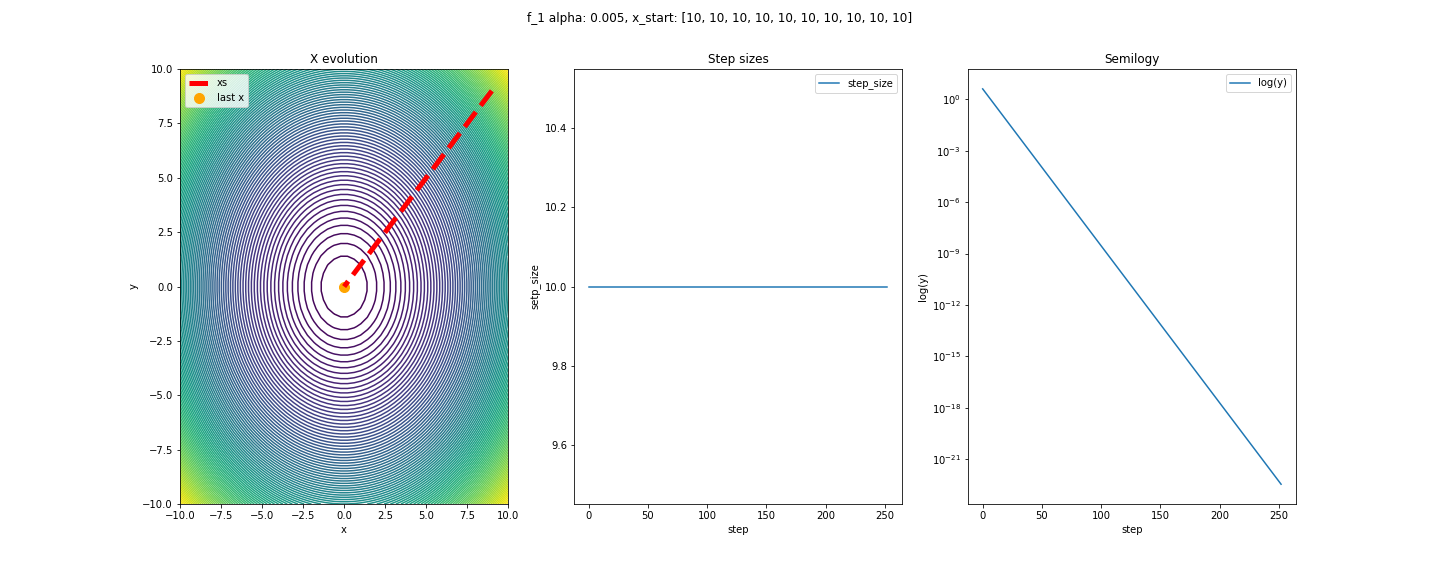
\includegraphics[width=\textwidth]{imgs/adaptatif_sz/f_1_a-0.005_adaptatif.png}
    \caption{}
\end{figure}
\begin{figure}[H]
    \centering
    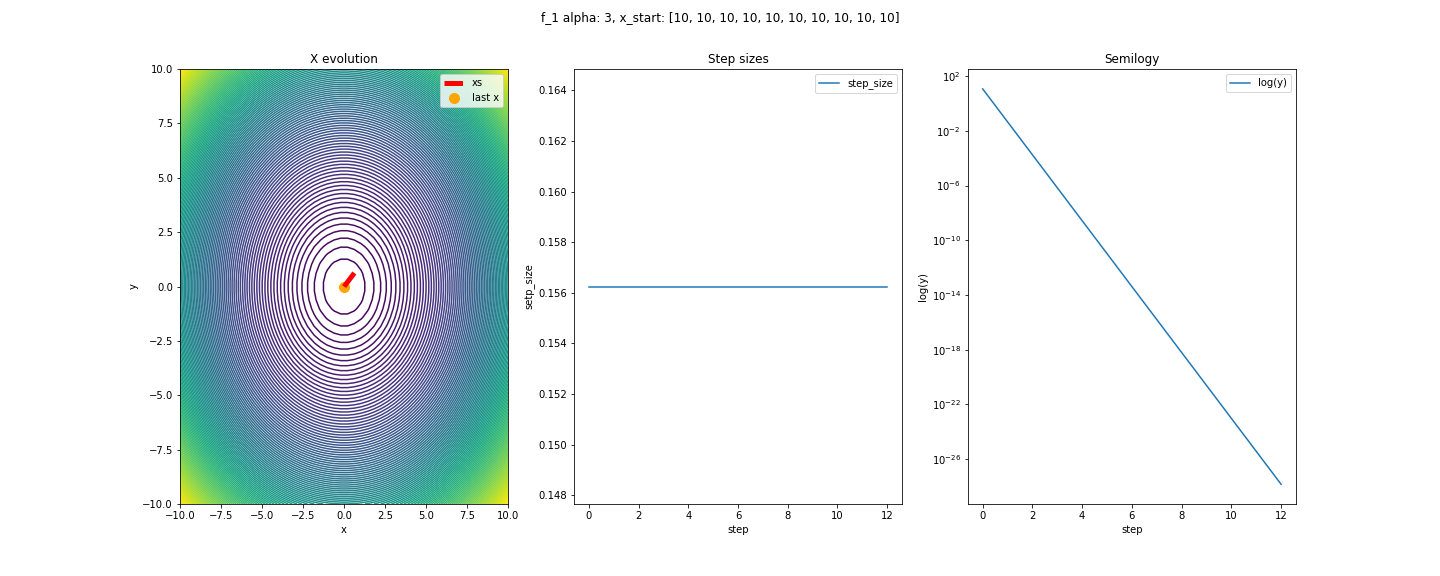
\includegraphics[width=\textwidth]{imgs/adaptatif_sz/f_1_a-3_adaptatif.png}
    \caption{}
\end{figure}
\begin{itemize}
	\item On remarque que le nombre d'itération est beaucoup moins élevé.
	\begin{itemize}
    	\item On converge beaucoup plus vite.
	\end{itemize}
\end{itemize}
\subsection{Fonction 2 }\label{sec:subsection2}
\begin{figure}[H]
    \centering
    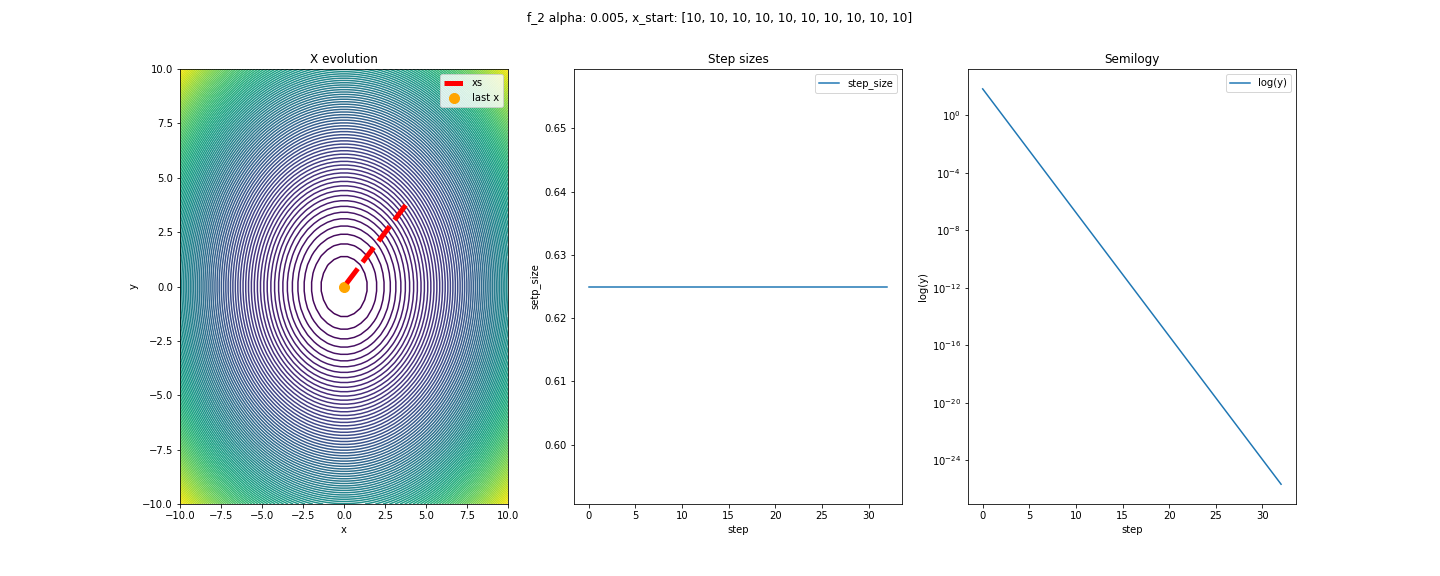
\includegraphics[width=\textwidth]{imgs/adaptatif_sz/f_2_a-0.005_adaptatif.png}
    \caption{}
\end{figure}
\begin{figure}[H]
    \centering
    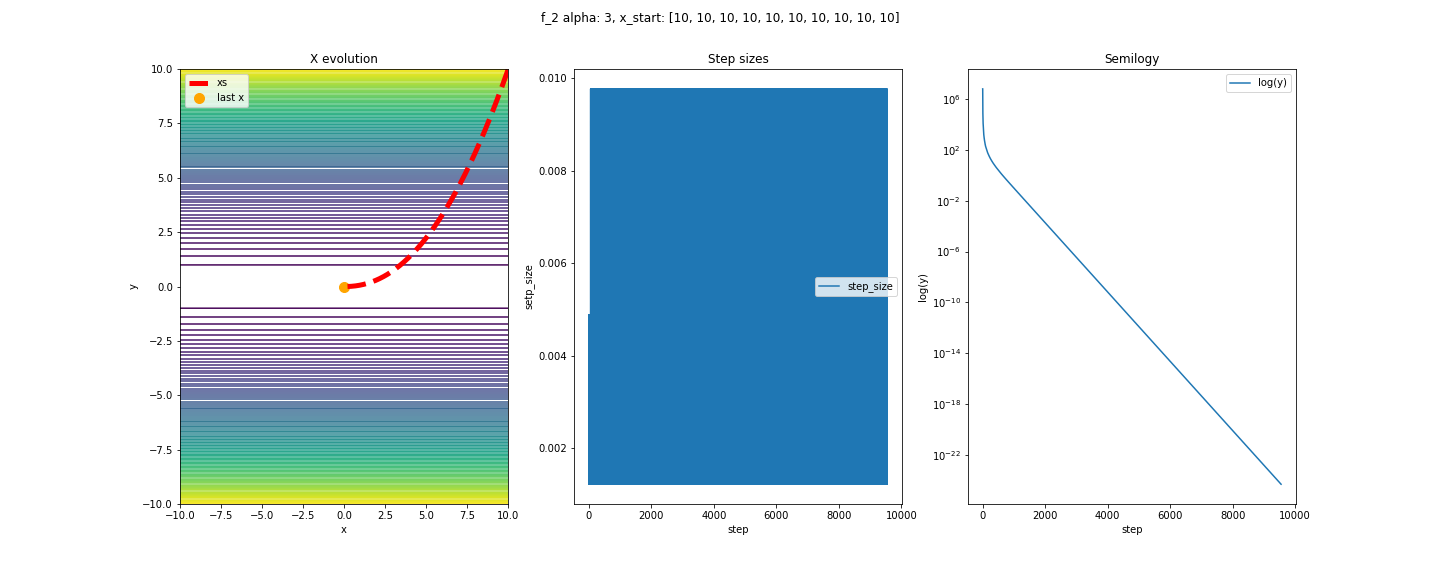
\includegraphics[width=\textwidth]{imgs/adaptatif_sz/f_2_a-3_adaptatif.png}
    \caption{}
\end{figure}
\begin{itemize}
	\item On remarque que le nombre d'itération est beaucoup moins élevé.
	\begin{itemize}
    	\item On converge beaucoup plus vite.
	\end{itemize}
	\item On remarque aussi que le step $step\_size$ oscille entre de faible valeurs $[0.02, 0.01]$.
\end{itemize}
\subsection{Fonction 3 }\label{sec:subsection2}
\begin{figure}[H]
    \centering
    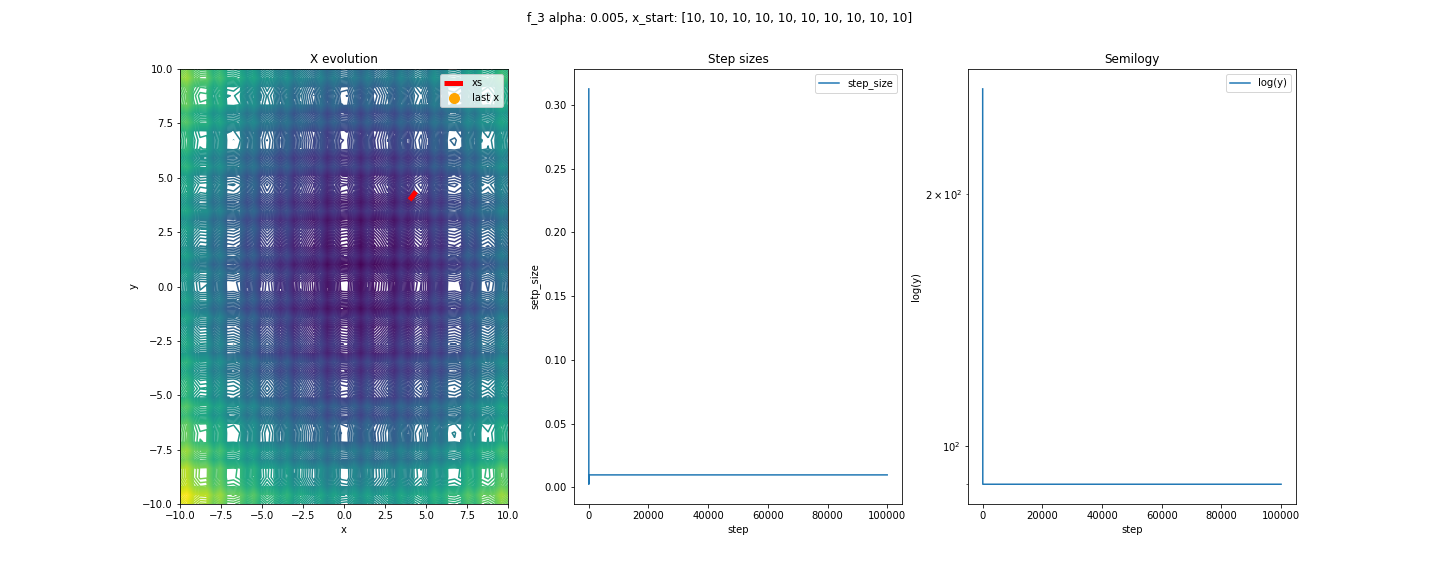
\includegraphics[width=\textwidth]{imgs/adaptatif_sz/f_3_a-0.005_adaptatif.png}
    \caption{}
\end{figure}
\begin{figure}[H]
    \centering
    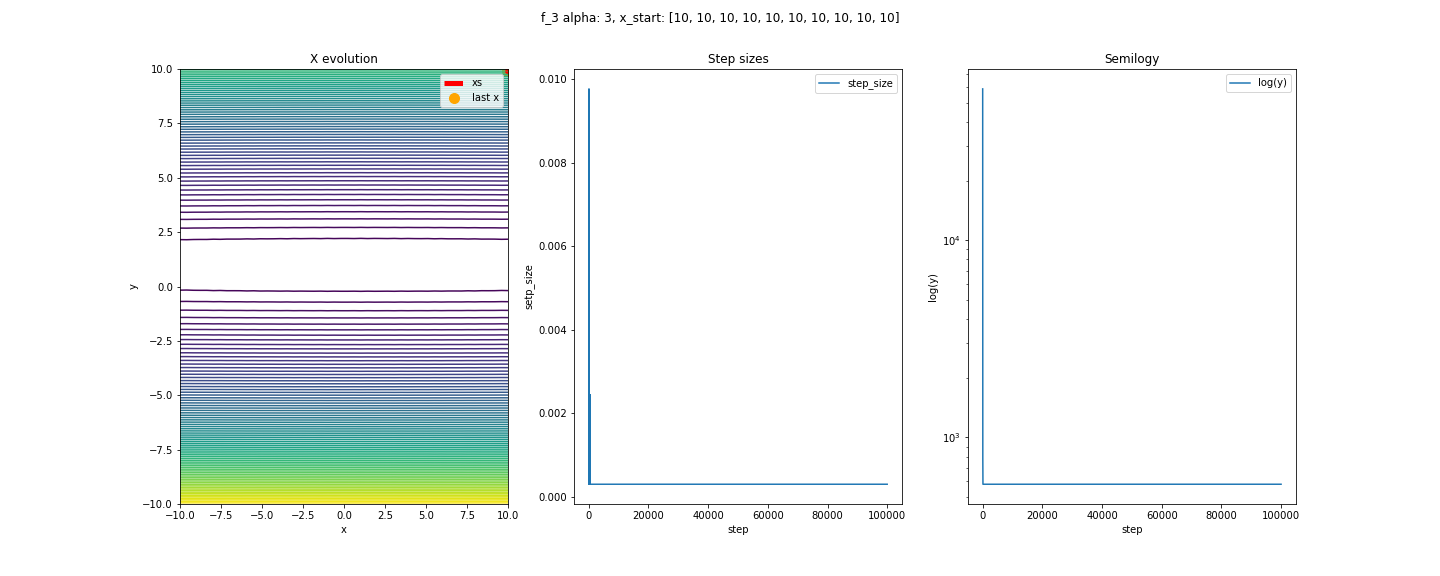
\includegraphics[width=\textwidth]{imgs/adaptatif_sz/f_3_a-3_adaptatif.png}
    \caption{}
\end{figure}
\begin{itemize}
	\item La fonction $f_3^{\alpha}(x)$ est plus complexe que les deux dernières (admet plusieurs minimums locaux).
	\item On remarque que l'agorithme peine à converger, on reste encore loin du minimum (0), malgrè un nombre élevé d'itération.
	\item On remarque aussi que le step $step\_size$ oscille entre de faible valeurs $[0.01, 0.02]$.

\end{itemize}
\subsection{Fonction 4 }\label{sec:subsection2}
\begin{figure}[H]
    \centering
    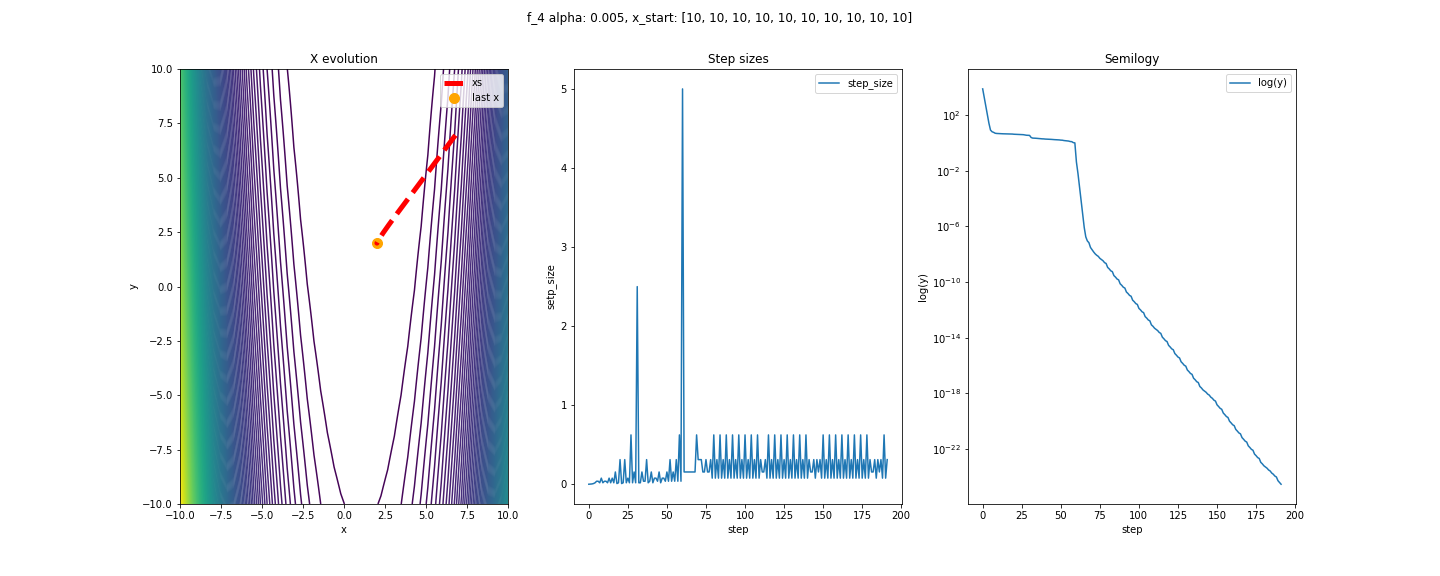
\includegraphics[width=\textwidth]{imgs/adaptatif_sz/f_4_a-0.005_adaptatif.png}
    \caption{}
\end{figure}
\begin{figure}[H]
    \centering
    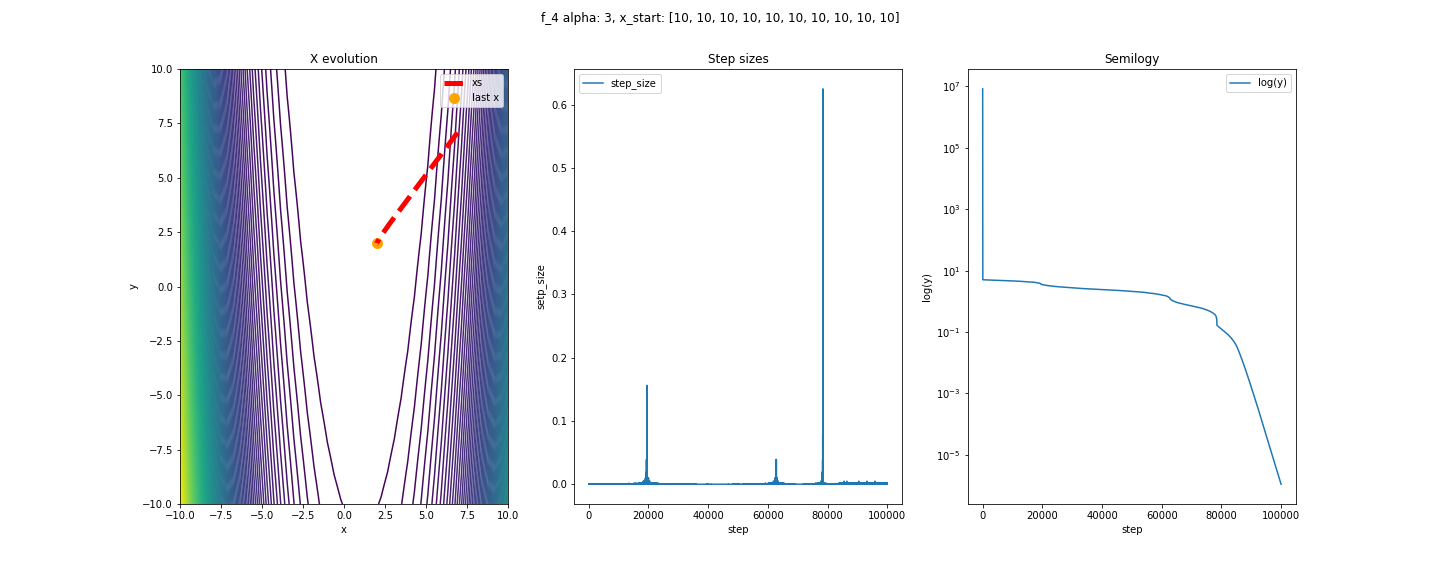
\includegraphics[width=\textwidth]{imgs/adaptatif_sz/f_4_a-3_adaptatif.png}
    \caption{}
\end{figure}
\begin{itemize}
	\item La fonction $f_4^{\alpha}(x)$ est la plus complexe (admet plusieurs minimums locaux).
	\item On remarque que l'agorithme peine à converger, on reste encore loin du minimum (0).
	\item On remarque aussi que le step $step\_size$ oscille entre des valeurs qui sont plus élevé que pour les fonctions précéentes $[0.6, 0.01]$.

\end{itemize}
% GD: NEWTON
\section{Gradient Descent: quasi-Newton Methode}\label{sec:section2}
Dans cette partie nous allons observer une descente de gradient avec la méthode quasi-Newton. Pour cela nous devons calcluer les dérivées seconde de chaque fonctions: 
\begin{equation}
    f_1''^{\alpha}(x) = 2.n.\alpha
    \label{eq:simple}		%these can be labelled too
\end{equation}
\begin{equation}
    f_2''(x) = n.10^{\alpha \frac {i-1} {n-1}}
    \label{eq:simple}		%these can be labelled too
\end{equation}
\begin{equation}
    f_3''(x) = \sum_{i=1}^{n} (2.10^{\alpha \frac {i-1} {n-1}} + 10.4\pi^{2}\cos(2\pi(x_i - 1)))
    \label{eq:simple}		%these can be labelled too
\end{equation}
\begin{sloppypar}
\begin{equation}
    f_4''(x) =
    \begin{cases} 
        \sum_{i=1}^{n} 4.10^{\alpha}.(xi - 1)  \\
        \sum_{i=1}^{n} -4.10^{\alpha}2.(x_i -1) 
    \end{cases}
    \label{eq:simple}		%these can be labelled too
\end{equation}
\end{sloppypar}
\subsection{Fonction 1 }\label{sec:subsection2}
\begin{figure}[H]
    \centering
    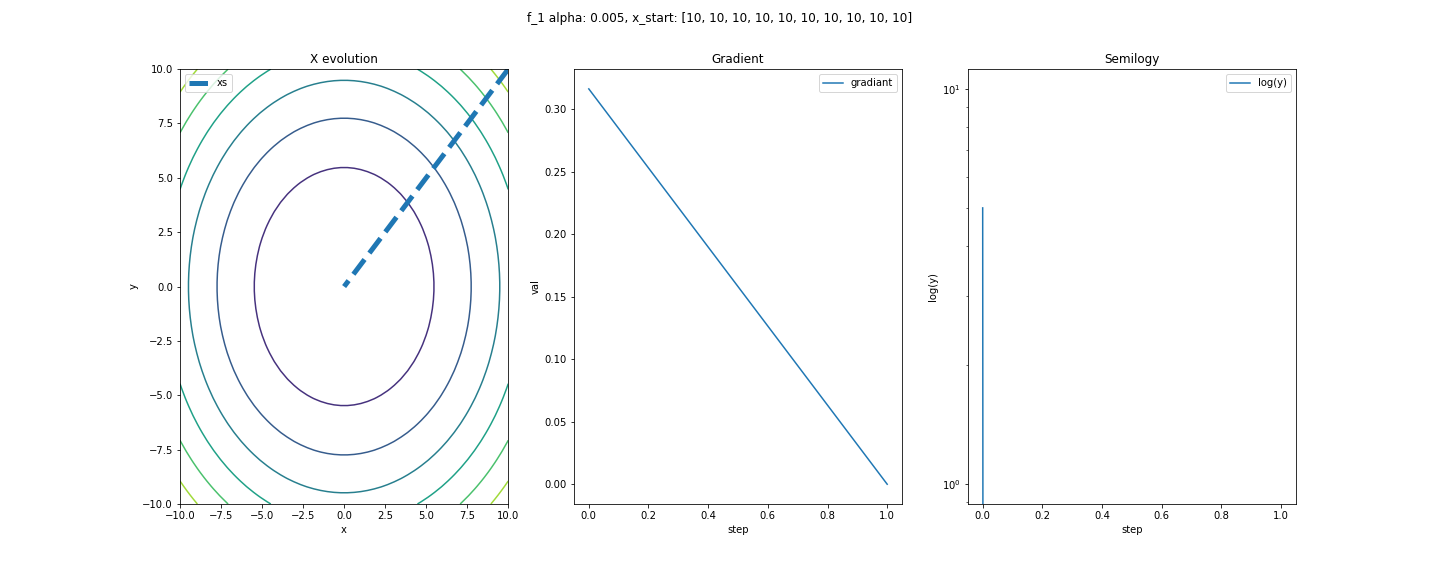
\includegraphics[width=\textwidth]{imgs/newton/f_1_a-0.005_newton.png}
    \caption{}
\end{figure}
\begin{figure}[H]
    \centering
    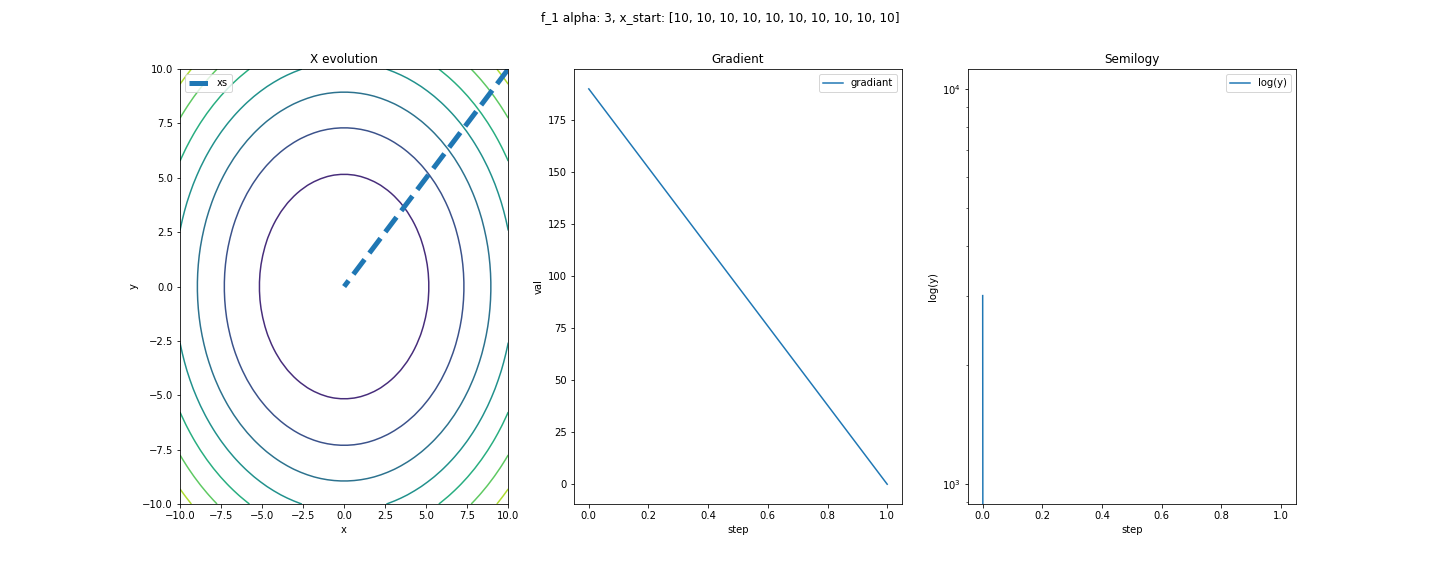
\includegraphics[width=\textwidth]{imgs/newton/f_1_a-3_newton.png}
    \caption{}
\end{figure}
\begin{itemize}
	\item La fonction $f_1^{\alpha}(x)$ reste assez simple (fonction convexe) ce qui permet de converger assez simplement.
	\item On peut remarquer ici que le facteur $\alpha$ impacte énormément sur la descente du gradiant.
	\begin{itemize}
    	\item Au plus $\alpha$ est grand, au plus le $step\_size$ doit être petit.
	\end{itemize}
\end{itemize}
\subsection{Fonction 2 }\label{sec:subsection2}
\begin{figure}[H]
    \centering
    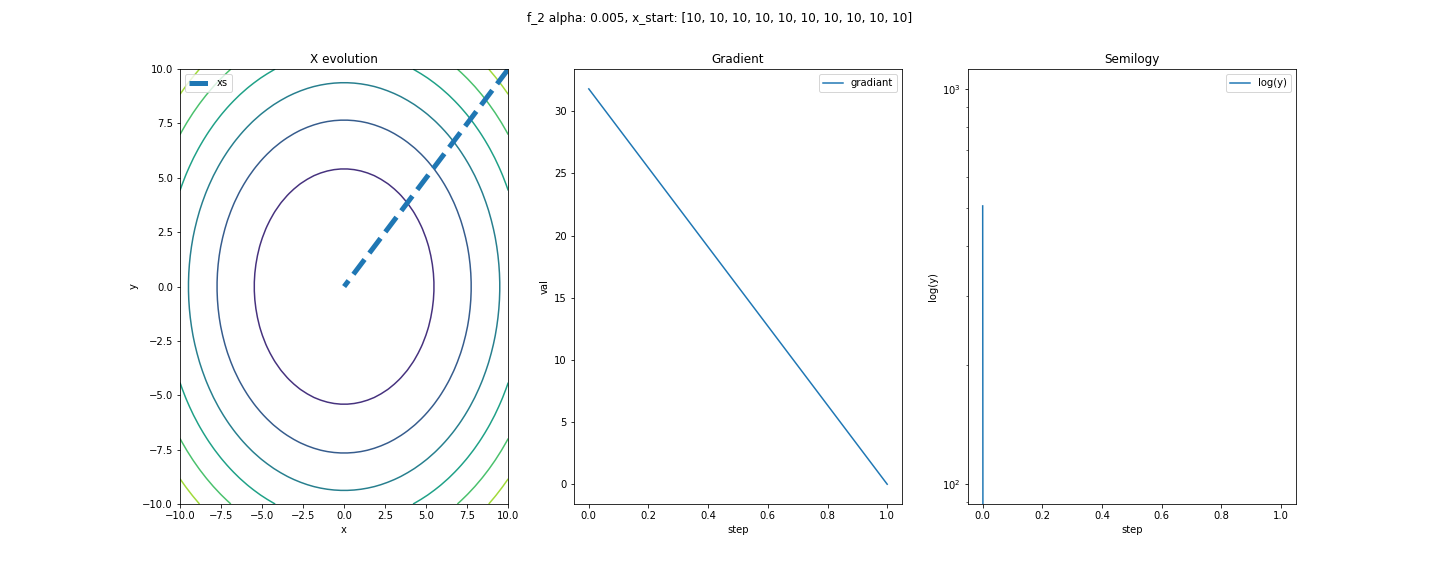
\includegraphics[width=\textwidth]{imgs/newton/f_2_a-0.005_newton.png}
    \caption{}
\end{figure}
\begin{figure}[H]
    \centering
    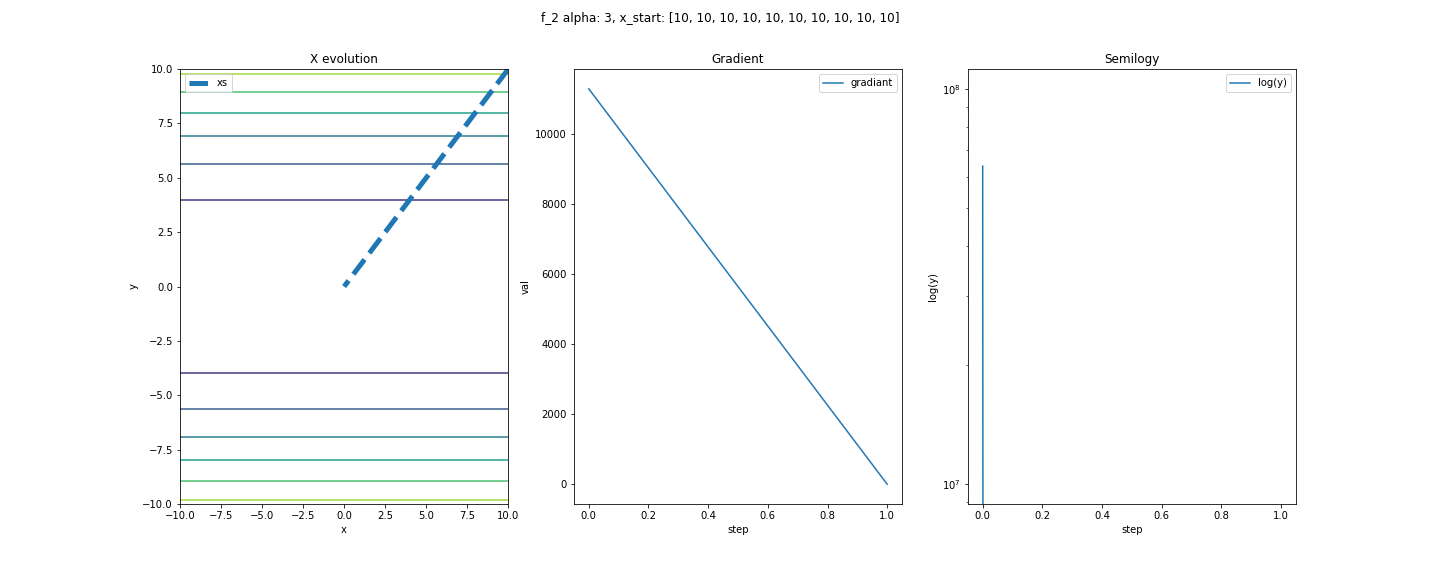
\includegraphics[width=\textwidth]{imgs/newton/f_2_a-3_newton.png}
    \caption{}
\end{figure}
\begin{itemize}
	\item La fonction $f_2^{\alpha}(x)$ reste assez simple (fonction convexe) ce qui permet de converger assez simplement.
	\item On peut remarquer ici que le facteur $\alpha$ impacte énormément la fonction et par suite impacte sur la descente du gradiant.
	\begin{itemize}
    	\item Au plus $\alpha$ est grand, au plus le $step\_size$ doit être petit.
	\end{itemize}
\end{itemize}
\subsection{Fonction 3 }\label{sec:subsection2}
\begin{figure}[H]
    \centering
    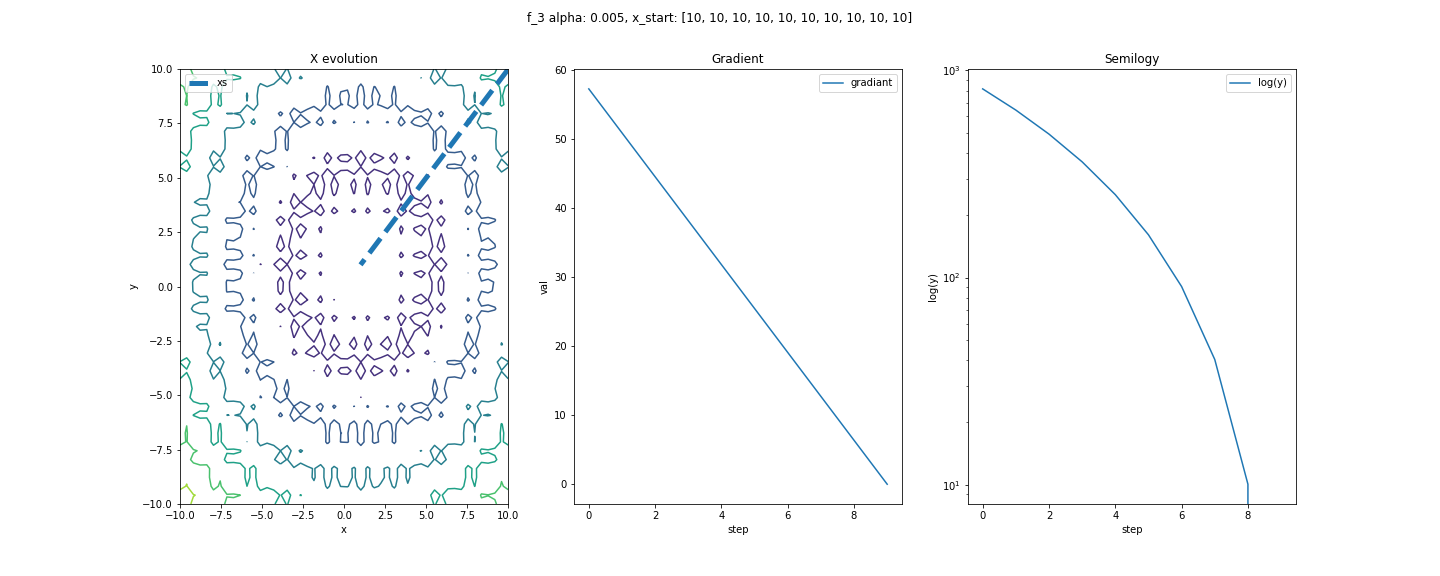
\includegraphics[width=\textwidth]{imgs/newton/f_3_a-0.005_newton.png}
    \caption{}
\end{figure}
\begin{figure}[H]
    \centering
    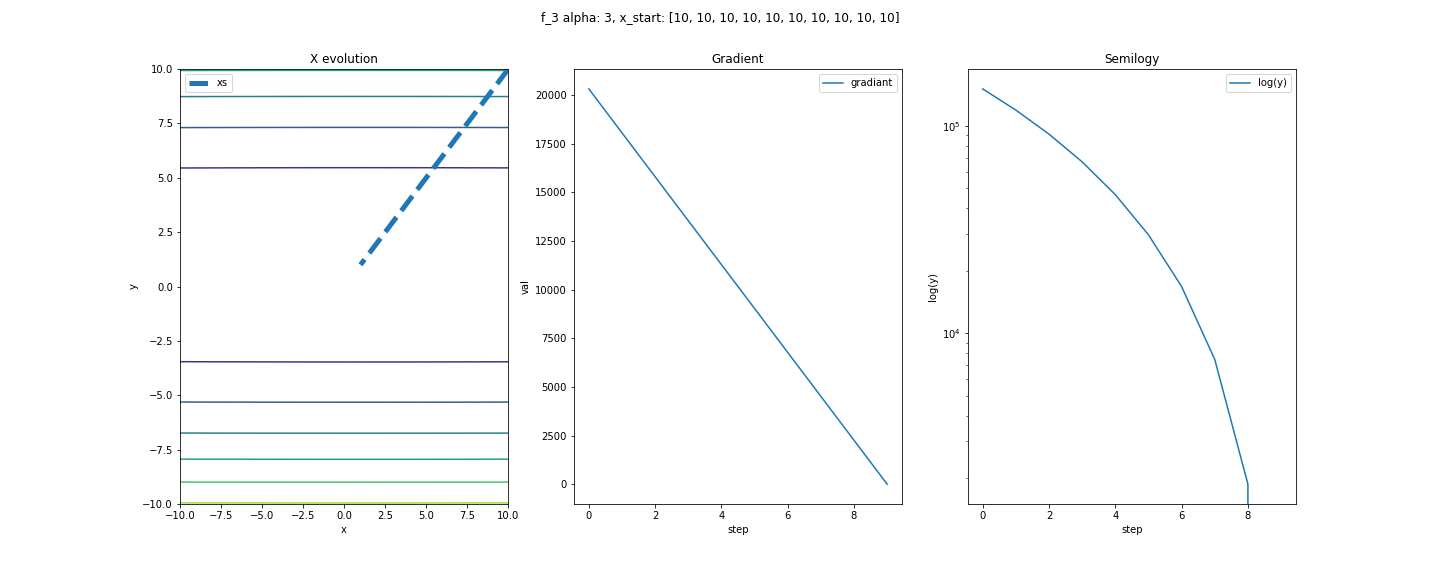
\includegraphics[width=\textwidth]{imgs/newton/f_3_a-3_newton.png}
    \caption{}
\end{figure}
\begin{itemize}
	\item La fonction $f_3^{\alpha}(x)$ est plus complexe que les deux dernières (admet plusieurs minimums locaux).
	\item On remarque que l'agorithme peine à converger, on reste encore loin du minimum (0).
	\item On peut remarquer ici que le facteur $\alpha$ impacte énormément la fonction et par suite impacte sur la descente du gradiant.
\end{itemize}
\subsection{Fonction 4 }\label{sec:subsection2}
\begin{figure}[H]
    \centering
    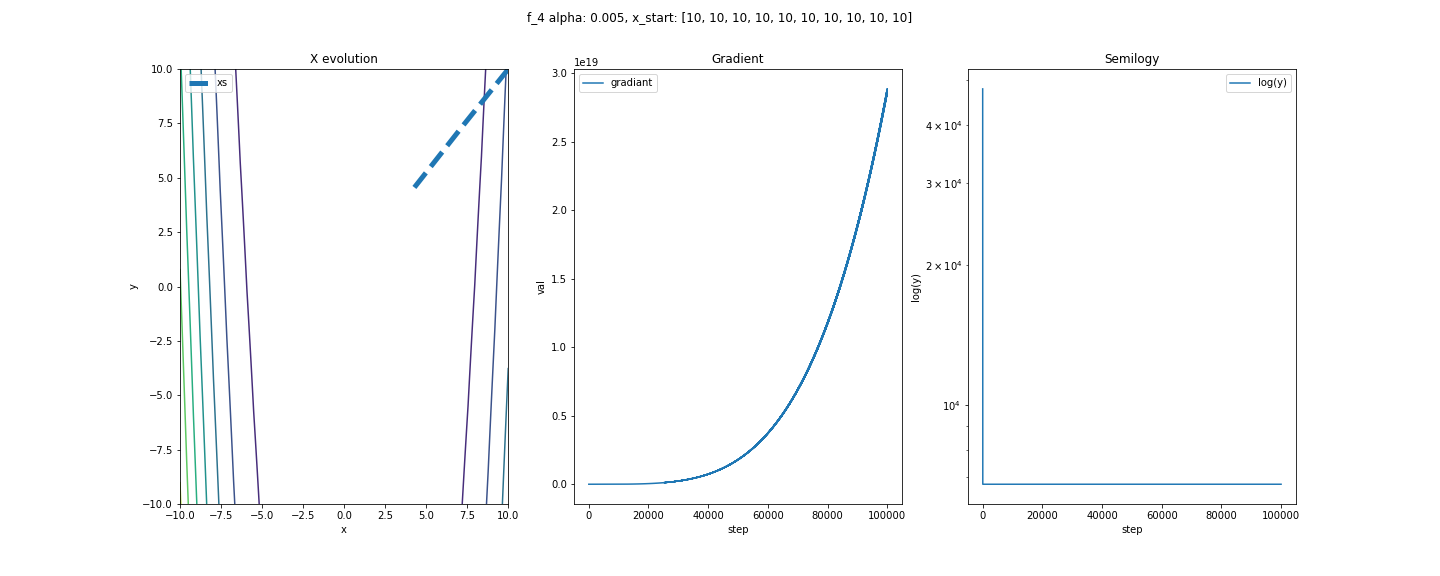
\includegraphics[width=\textwidth]{imgs/newton/f_4_a-0.005_newton.png}
    \caption{}
\end{figure}
\begin{figure}[H]
    \centering
    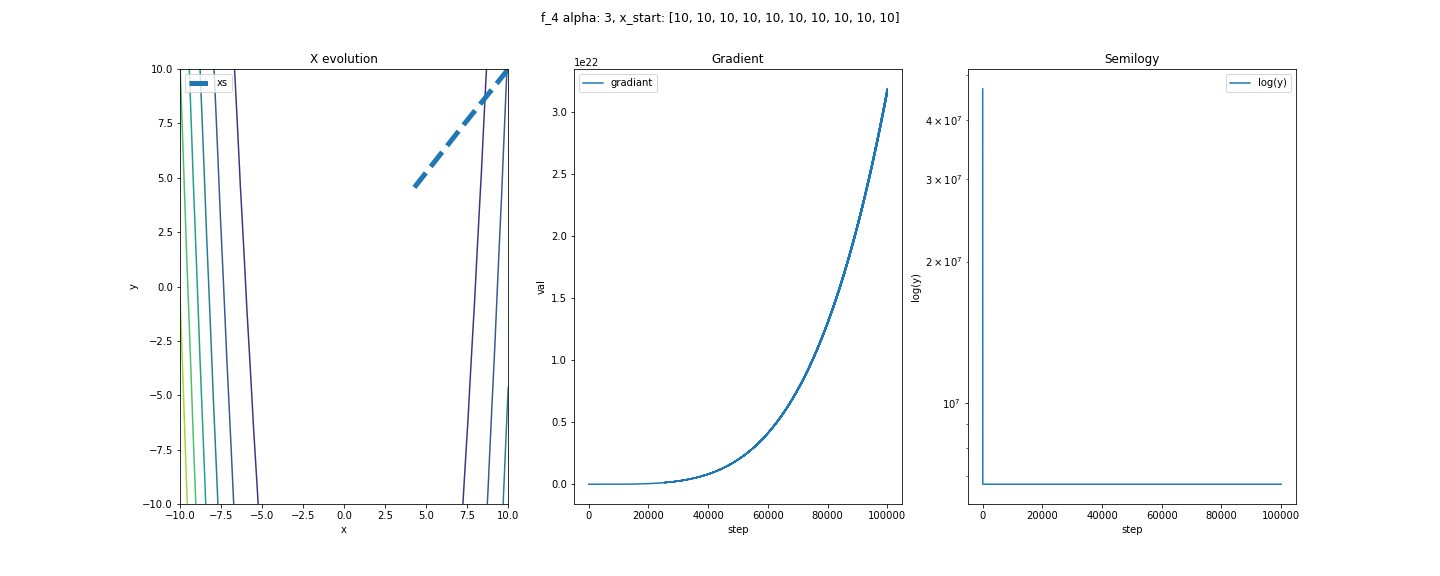
\includegraphics[width=\textwidth]{imgs/newton/f_4_a-3_newton.png}
    \caption{}
\end{figure}
\begin{itemize}
	\item La fonction $f_4^{\alpha}(x)$ est la plus complexe (admet plusieurs minimums locaux).
	\item On remarque que l'agorithme peine à converger, on reste encore loin du minimum (0).
\end{itemize}



% Comparaison: NEWTON
\section{Comparaison Newton VS BFGS}\label{sec:section2}
Dans cette partie nous comparer la méthode Newton à la méthode BFGS de la bilothéque scipy.

\subsection{Fonction 1 }\label{sec:subsection2}
\begin{figure}[H]
    \centering
    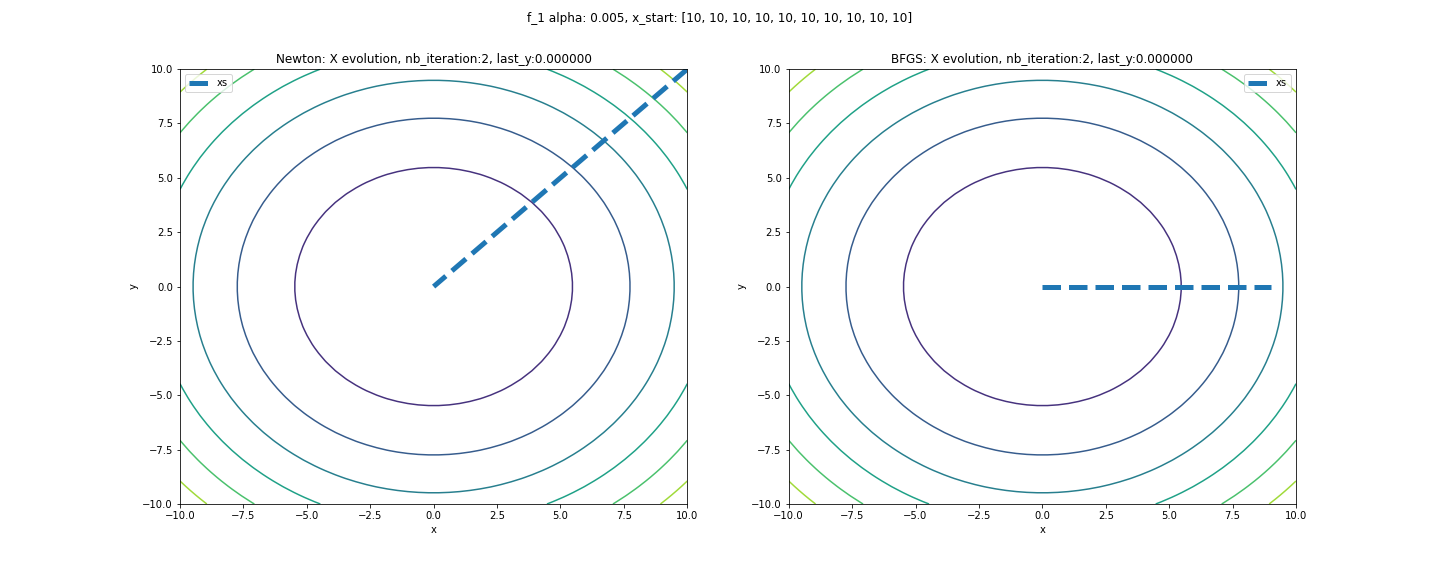
\includegraphics[width=\textwidth]{imgs/comparaison/f_1_a-0.005.png}
    \caption{}
\end{figure}
\begin{figure}[H]
    \centering
    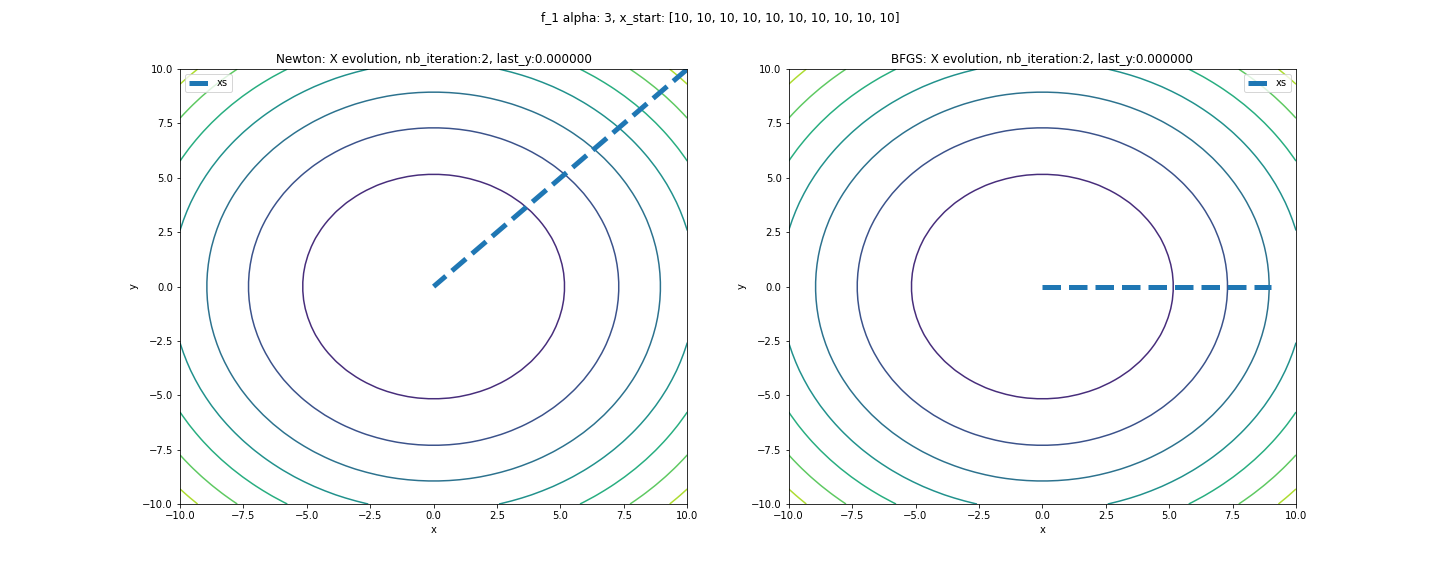
\includegraphics[width=\textwidth]{imgs/comparaison/f_1_a-3.png}
    \caption{}
\end{figure}
\begin{itemize}
	\item On peut remarquer ici que les deux méthodes sont équivalentes.
\end{itemize}
\subsection{Fonction 2 }\label{sec:subsection2}
\begin{figure}[H]
    \centering
    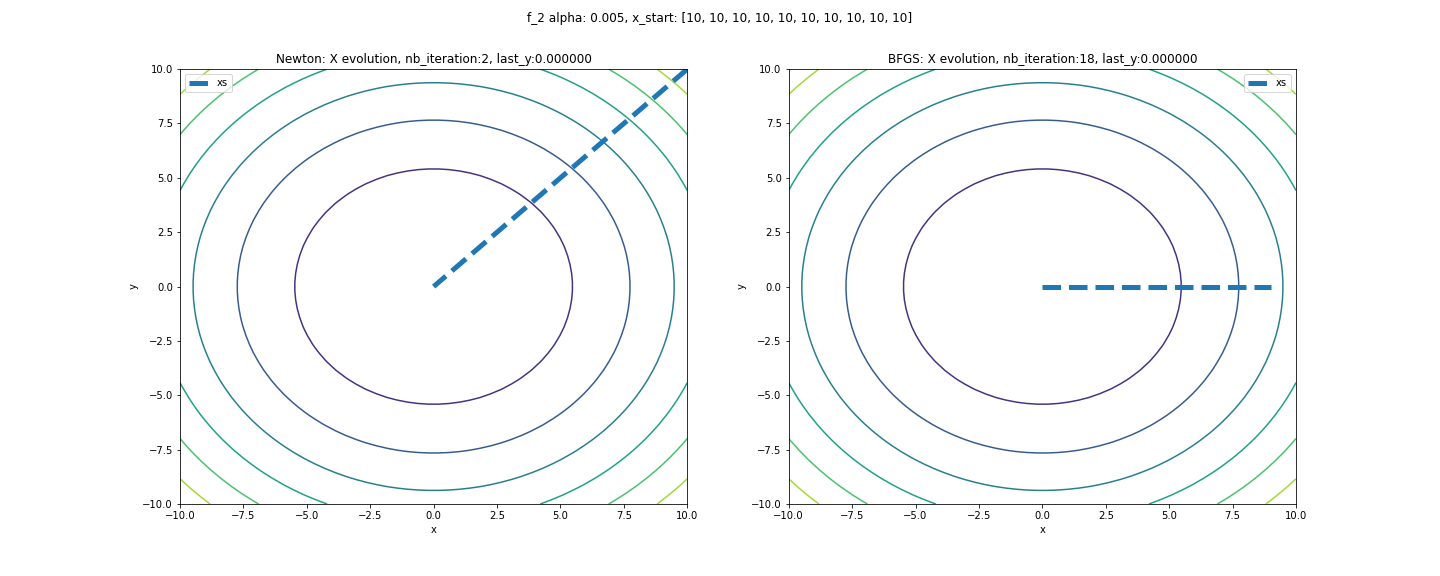
\includegraphics[width=\textwidth]{imgs/comparaison/f_2_a-0.005.png}
    \caption{}
\end{figure}
\begin{figure}[H]
    \centering
    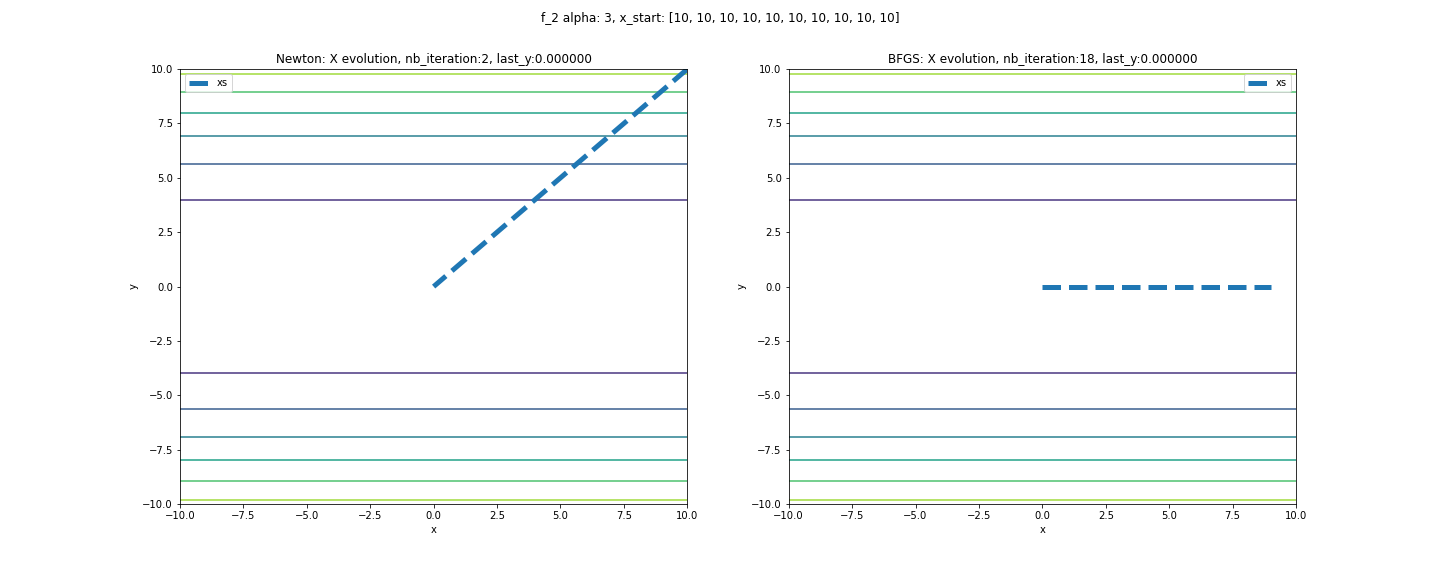
\includegraphics[width=\textwidth]{imgs/comparaison/f_2_a-3.png}
    \caption{}
\end{figure}
\begin{itemize}
	\item On peut remarquer ici que les deux méthodes sont équivalentes.
\end{itemize}
\subsection{Fonction 3 }\label{sec:subsection2}
\begin{figure}[H]
    \centering
    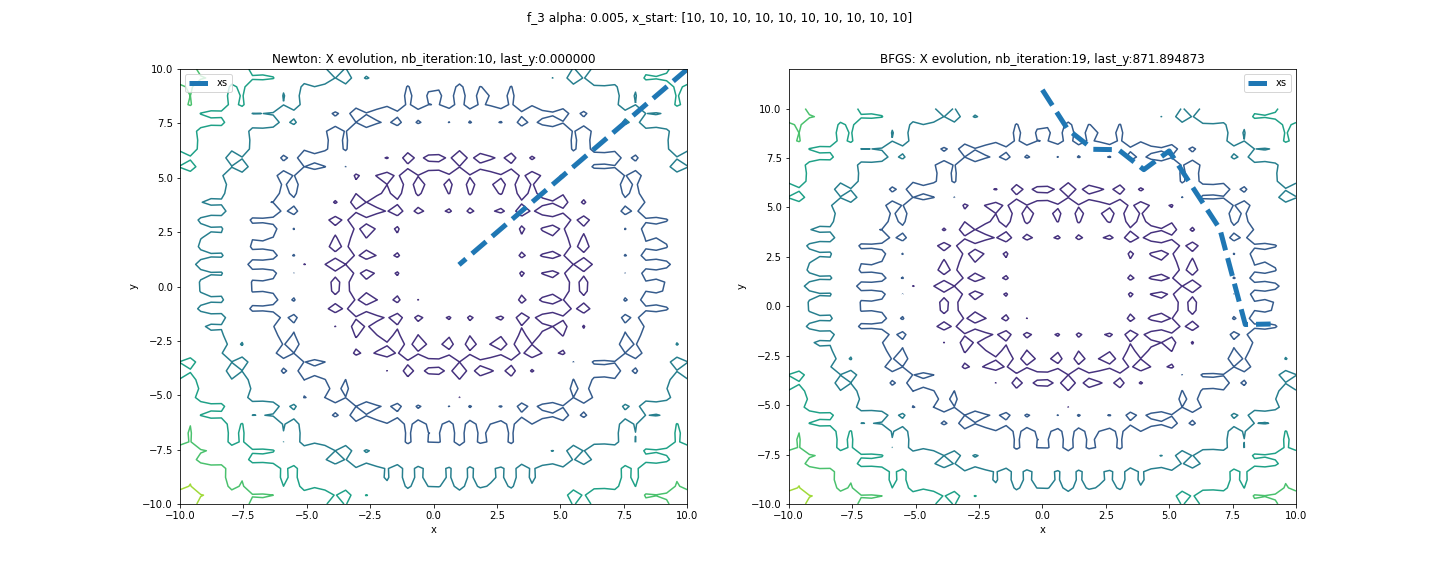
\includegraphics[width=\textwidth]{imgs/comparaison/f_3_a-0.005.png}
    \caption{}
\end{figure}
\begin{figure}[H]
    \centering
    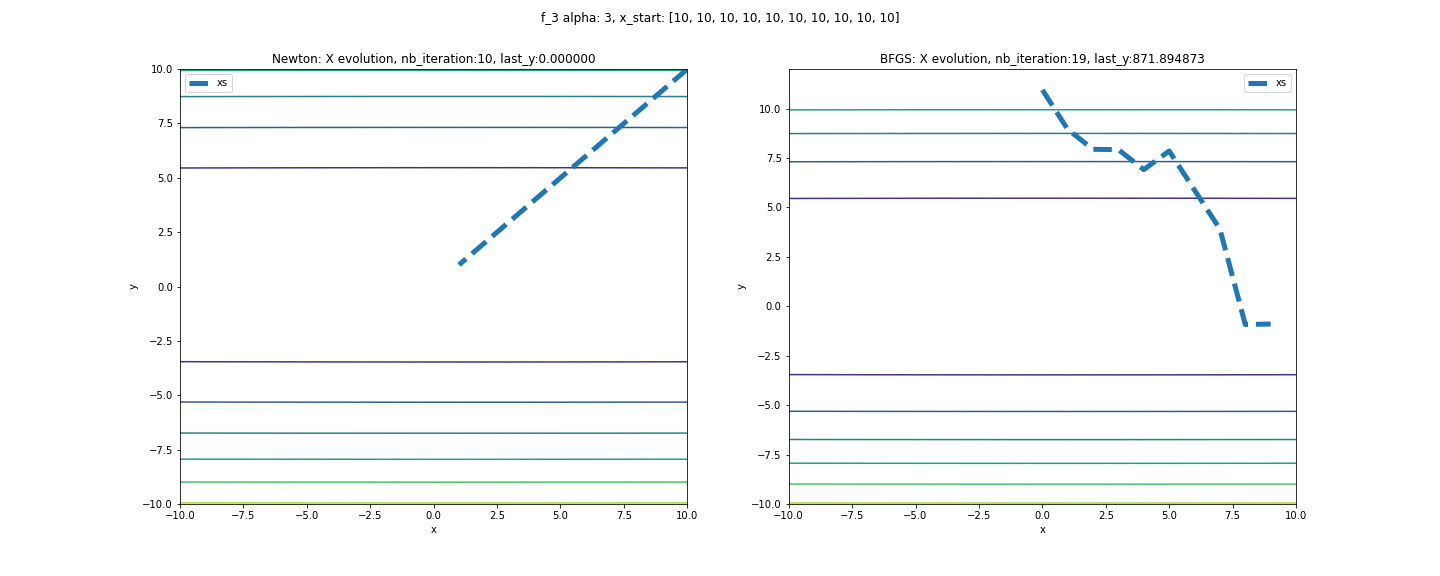
\includegraphics[width=\textwidth]{imgs/comparaison/f_3_a-3.png}
    \caption{}
\end{figure}
\begin{itemize}
	\item On peut remarquer ici que la méthode Newton est meilleur que BFGS.
\end{itemize}
\subsection{Fonction 4 }\label{sec:subsection2}
\begin{figure}[H]
    \centering
    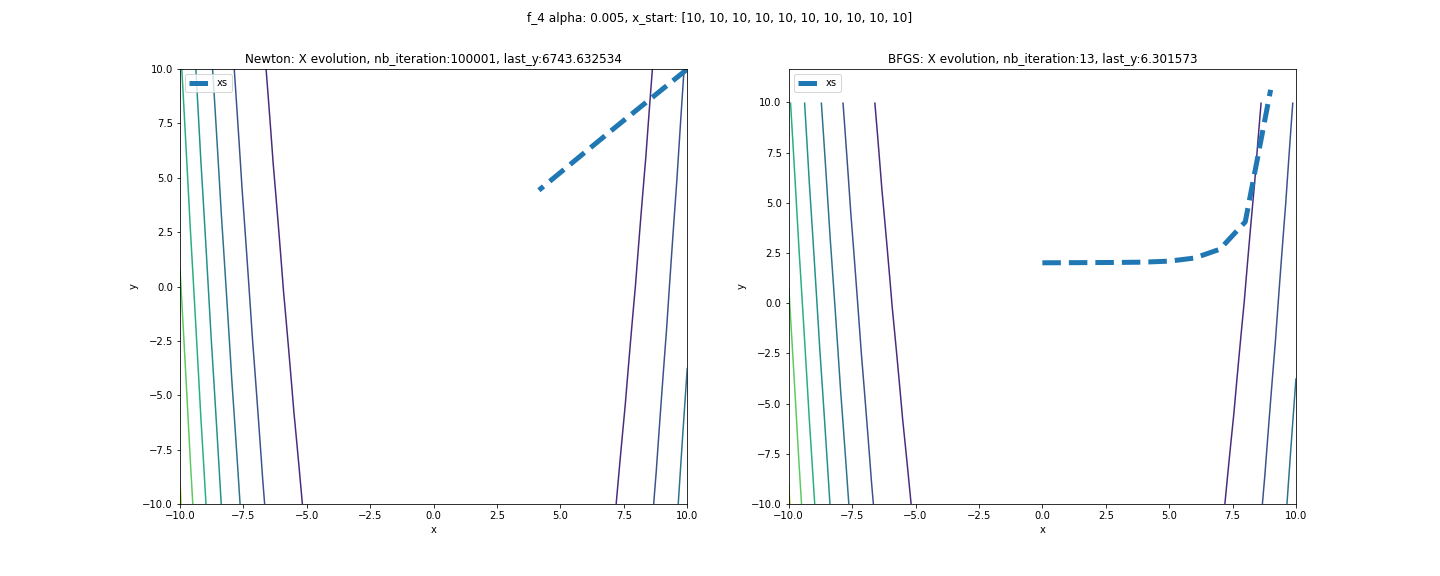
\includegraphics[width=\textwidth]{imgs/comparaison/f_4_a-0.005.png}
    \caption{}
\end{figure}
\begin{figure}[H]
    \centering
    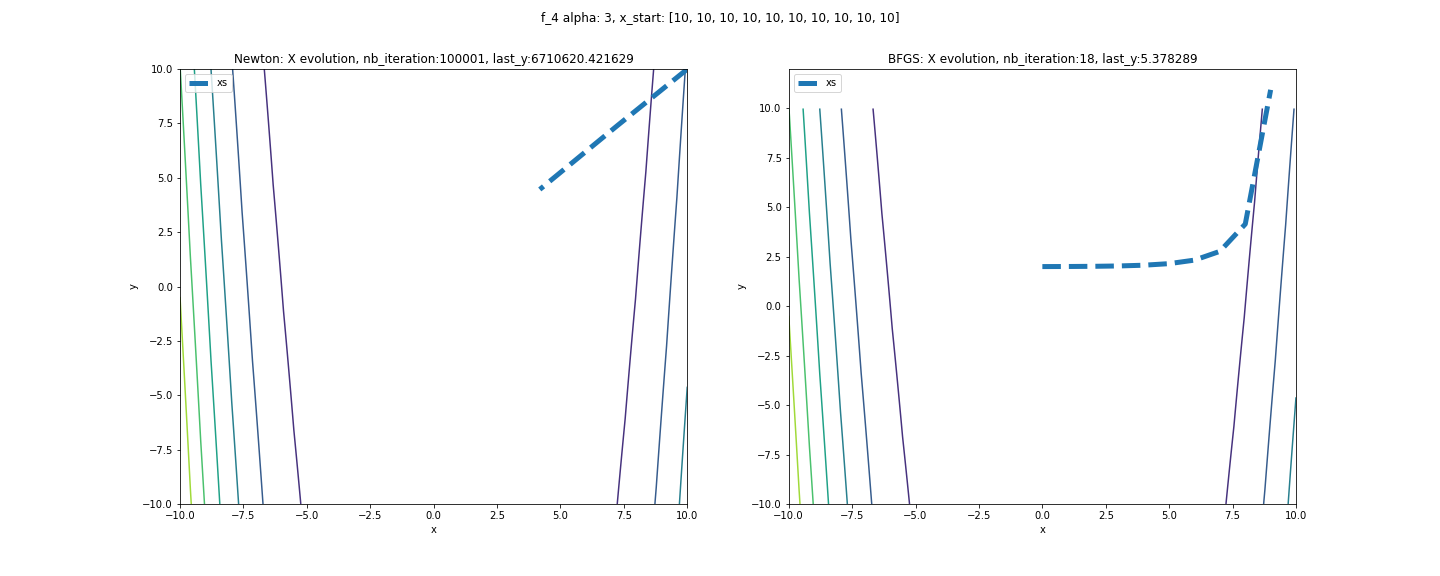
\includegraphics[width=\textwidth]{imgs/comparaison/f_4_a-3.png}
    \caption{}
\end{figure}
\begin{itemize}
	\item On peut remarquer ici que la methode BFGS est meilleur que Newton.
\end{itemize}


\end{document}
